\documentclass[11pt,]{book}
\usepackage{lmodern}
\usepackage{amssymb,amsmath}
\usepackage{ifxetex,ifluatex}
\usepackage{fixltx2e} % provides \textsubscript
\ifnum 0\ifxetex 1\fi\ifluatex 1\fi=0 % if pdftex
  \usepackage[T1]{fontenc}
  \usepackage[utf8]{inputenc}
\else % if luatex or xelatex
  \ifxetex
    \usepackage{mathspec}
  \else
    \usepackage{fontspec}
  \fi
  \defaultfontfeatures{Ligatures=TeX,Scale=MatchLowercase}
\fi
% use upquote if available, for straight quotes in verbatim environments
\IfFileExists{upquote.sty}{\usepackage{upquote}}{}
% use microtype if available
\IfFileExists{microtype.sty}{%
\usepackage{microtype}
\UseMicrotypeSet[protrusion]{basicmath} % disable protrusion for tt fonts
}{}
\usepackage[margin=1in]{geometry}
\usepackage{hyperref}
\hypersetup{unicode=true,
            pdfborder={0 0 0},
            breaklinks=true}
\urlstyle{same}  % don't use monospace font for urls
\usepackage{longtable,booktabs}
\usepackage{graphicx,grffile}
\makeatletter
\def\maxwidth{\ifdim\Gin@nat@width>\linewidth\linewidth\else\Gin@nat@width\fi}
\def\maxheight{\ifdim\Gin@nat@height>\textheight\textheight\else\Gin@nat@height\fi}
\makeatother
% Scale images if necessary, so that they will not overflow the page
% margins by default, and it is still possible to overwrite the defaults
% using explicit options in \includegraphics[width, height, ...]{}
\setkeys{Gin}{width=\maxwidth,height=\maxheight,keepaspectratio}
\IfFileExists{parskip.sty}{%
\usepackage{parskip}
}{% else
\setlength{\parindent}{0pt}
\setlength{\parskip}{6pt plus 2pt minus 1pt}
}
\setlength{\emergencystretch}{3em}  % prevent overfull lines
\providecommand{\tightlist}{%
  \setlength{\itemsep}{0pt}\setlength{\parskip}{0pt}}
\setcounter{secnumdepth}{5}
% Redefines (sub)paragraphs to behave more like sections
\ifx\paragraph\undefined\else
\let\oldparagraph\paragraph
\renewcommand{\paragraph}[1]{\oldparagraph{#1}\mbox{}}
\fi
\ifx\subparagraph\undefined\else
\let\oldsubparagraph\subparagraph
\renewcommand{\subparagraph}[1]{\oldsubparagraph{#1}\mbox{}}
\fi

%%% Use protect on footnotes to avoid problems with footnotes in titles
\let\rmarkdownfootnote\footnote%
\def\footnote{\protect\rmarkdownfootnote}

%%% Change title format to be more compact
\usepackage{titling}

% Create subtitle command for use in maketitle
\newcommand{\subtitle}[1]{
  \posttitle{
    \begin{center}\large#1\end{center}
    }
}

\setlength{\droptitle}{-2em}
  \title{}
  \pretitle{\vspace{\droptitle}}
  \posttitle{}
  \author{}
  \preauthor{}\postauthor{}
  \date{}
  \predate{}\postdate{}

\newlength{\drop}
\usepackage{booktabs}
\usepackage{longtable}
\usepackage{emptypage}
\usepackage[table]{xcolor}
\usepackage{array}
\usepackage{multirow}
\usepackage{wrapfig}
\usepackage{float}
\usepackage{colortbl}
\usepackage{pdflscape}
\usepackage{tabu}
\usepackage{threeparttable}
\usepackage[normalem]{ulem}
\usepackage{rotating}
\renewcommand{\textfraction}{0.05}
\renewcommand{\topfraction}{0.8}
\renewcommand{\bottomfraction}{0.8}
\renewcommand{\floatpagefraction}{0.75}
\raggedbottom

\usepackage{amsthm}
\newtheorem{theorem}{Theorem}[chapter]
\newtheorem{lemma}{Lemma}[chapter]
\theoremstyle{definition}
\newtheorem{definition}{Definition}[chapter]
\newtheorem{corollary}{Corollary}[chapter]
\newtheorem{proposition}{Proposition}[chapter]
\theoremstyle{definition}
\newtheorem{example}{Example}[chapter]
\theoremstyle{definition}
\newtheorem{exercise}{Exercise}[chapter]
\theoremstyle{remark}
\newtheorem*{remark}{Remark}
\newtheorem*{solution}{Solution}
\begin{document}

\begin{titlepage}
	\drop=0.1\textheight
	\centering
	\vspace*{\baselineskip}
	\rule{\textwidth}{1.6pt}\vspace*{-\baselineskip}\vspace*{2pt}
	\rule{\textwidth}{0.4pt}\\[\baselineskip]
	{\Large FARM MANAGEMENT\\[1.2\baselineskip] and \\[1.2\baselineskip] MARKETING}\\[1.2\baselineskip]
	\rule{\textwidth}{0.4pt}\vspace*{-\baselineskip}\vspace{3.2pt}
	\rule{\textwidth}{1.6pt}\\[\baselineskip]
	\scshape
	Notes handout \\ % reasonable subtitle
	\vspace*{3\baselineskip}
	Edited by \\[\baselineskip]
	{\Large Deependra Dhakal\par} % insert any number of editors by following with "\\" after first
	% {\Large Deependra Dhakal \\ Deependra Dhakal\par} % example multieditors
	{\itshape Instructor \\ Triveni Secondary School \\ Katari, Udayapur\par} % typically organization name and address
	\vfill
	{\scshape 2018} \\
	% {\Large Publisher name}\par % contains publisher name
\end{titlepage}

{
\setcounter{tocdepth}{2}
\tableofcontents
}
\chapter*{Background}\label{background}
\addcontentsline{toc}{chapter}{Background}

The handout is intended for students trying to have basic starting idea
on the course of economics. An agricultural economics based approach is
taken, to delve in to the concepts of Micro and Macro economics. The
note is expected to be helpful to students preparing for upper and lower
secondary level examinations.

While teaching Farm Management and Marketing course, I felt the
necessity to deliver contents to students in a broad context, afterall
farm mangement is just a part wider field of economics. The question
solution approach to this note should provide succinct answers to, as
well as a more elaborate exposition in a follow through, conceptual
questions surrounding the applied course. The contents presented here,
however, do not form a sound basis for practical understanding.

\part{Questions}\label{part-questions}

\textbf{Economics and international trade questions}

\begin{itemize}
\tightlist
\item
  State Adam Smiths' definition of economics.
\item
  Define cost.
\item
  What is income statement?
\item
  Give an example of monopoly market.
\item
  What is Farm Planning?
\item
  What is Agriculture Marketing?
\item
  What are the types of utility? Give examples.
\item
  State the law of supply. Describe with the help of supply curve
  diagram.
\item
  What are the characteristics of perfect competition market?
\item
  What do you mean by price variation? Describe with examples.
\item
  What are the functions of WTO?
\item
  Explain the principle of substitution.
\item
  Write the importance of farm plan.
\item
  What do you mean by Net-worth statement?
\item
  Give the differences between complete and partial budgeting.
\item
  Agriculture commodities are seasonal in nature. Justify.
\item
  What are the selection criteria of best channel for distribution of
  agriculture commodities.
\item
  Write the characteristics of the material welfare definition of
  economics.
\item
  Explain in detail about the farm record.
\item
  What are the objectives of farm management?
\item
  State the law of demand with its assumptions. Give a description with
  suitable examples.
\item
  Define farm management. Highlight its importance.
\item
  Explain the principle of product substitution in detail.
\item
  Explain in detail about farm efficiency measures.
\item
  Describe the role of cooperatives in Nepalese economy.
\item
  Classify markets of Nepal on different basis.
\item
  What is a marketing channel? Explain with suitable examples.
\item
  Define capital.
\item
  Define cooperative farming.
\item
  What is marketing margin?
\item
  What is a whole sale market?
\item
  Write the features of land.
\item
  What are the problems of farm record keeping in Nepal?
\item
  Explain the law of diminishing marginal utility.
\item
  Write the properties of indifference curve with examples.
\item
  What is market?
\item
  Explain the importance of agricultural marketing in socio-economic
  development of Nepal.
\item
  Write notes on following topics:

  \begin{itemize}
  \tightlist
  \item
    Goods
  \item
    Labor
  \item
    Wealth
  \item
    Service
  \item
    Equilibrium
  \item
    Price line
  \end{itemize}
\item
  What is meant by elasticity of supply?
\end{itemize}

\textbf{Agricultural marketing questions}

\begin{itemize}
\tightlist
\item
  What is Agriculture Marketing?
\item
  What are the selection criteria of best channel for distribution of
  agriculture commodities.
\item
  Classify markets of Nepal on different basis.
\item
  What is a marketing channel? Explain with suitable examples.
\item
  What is marketing margin?
\item
  What is a whole sale market?
\item
  What is market?
\item
  Explain the importance of agricultural marketing in socio-economic
  development of Nepal.
\item
  Describe the role of cooperatives in Nepalese economy.
\end{itemize}

\part{Course matter}\label{part-course-matter}

\chapter{Economics and international
trade}\label{economics-and-international-trade}

\section{Economics: meaning and
definition}\label{economics-meaning-and-definition}

An economy is a system for coordinating society's productive activities.

\begin{itemize}
\tightlist
\item
  Economics is the social science that studies the production,
  distribution, and consumption of goods and services.
\item
  Economics is the study of individual choices and decisions. People
  must make choices because resources are scarce.
\end{itemize}

\begin{quote}
\textbf{Microeconomics} \newline The branch of economics that studies
how people make decisions and how these decisions interact.
\end{quote}

\begin{quote}
\textbf{Macroeconomics} \newline The branch of economics that is
concerned with overall ups and downs in the economy.
\end{quote}

The objective of microeconomics are:

\begin{enumerate}
\def\labelenumi{\arabic{enumi}.}
\tightlist
\item
  Economic efficiency: productive efficiency, consumptive efficiency and
  allocative efficiency
\item
  Equity: A distribution of income that is considered to be fair or
  just.
\end{enumerate}

The discipline of economics has developed principles, theories, and
models that isolate the most important determinants of economic events.
In constructing a model, economists make assumptions to eliminate
unnecessary detail to reduce the complexity of economic behavior. Once
modeled, economic behavior may be presented as a relationship between
dependent and independent variables. The behavior being explained is the
dependent variable; the economic events explaining that behavior are the
independent variables.The dependent variable may be presented as
depending upon one independent variable, with the influence of the other
independent variables held constant (the \emph{ceteris paribus}
assumption).

\subsection{Problem of scarcity}\label{problem-of-scarcity}

Economics is the study of scarcity-- the study of the allocation of
scarce resources to satisfy human wants. People's material wants, for
the most part, are unlimited. Output, on the other hand, is limited by
the state of technology and the quantity and quality of the economy's
resources. Thus, the production of each good and service involves a
cost. A \textbf{good} is usually defined as a physical item such as a
car or a hamburger, and a service is something provided to you such as
insurance or a haircut. Scarcity is a fundamental problem for every
society. Decisions must be made regarding \emph{what to produce},
\emph{how to produce} it, and \emph{for whom to produce}. What to
produce involves decisions about the kinds and quantities of goods and
services to produce. How to produce requires decisions about what
techniques to use and how economic resources (or factors of production)
are to be combined in producing output.

\subsection{Positive and normative
economics}\label{positive-and-normative-economics}

Positive questions have to do with explanation and prediction, normative
questions with what ought to be. Positive and normative economics are
often synthesized in the style of practical idealism. In this
discipline, sometimes called the ``art of economics,'' positive
economics is utilized as a practical tool for achieving normative
objectives.

\subsubsection{Positive economics}\label{positive-economics}

Positive economics tries to reason the cause and effect of an economic
activity. Questions such as ``What will happen if?'' and ``What impact
will it have on'' are all in the realm of positive analysis. Positive
analysis is central to microeconomics. Theories are developed to explain
phenomena, are tested against observations, and are used to construct
models from which predictions are made.

The use of economic theory for prediction is important both for the
managers of firms and for public policy. Suppose the federal government
is considering raising the tax on gasoline. The tax would affect the
price of gasoline, consumers' preferences for small or large cars, the
amount of driving that people do, and so on. To plan sensibly, oil
companies, automobile companies, producers of automobile parts, and
firms in the tourist industry would all want to know how large the
various effects of this tax will be. Government policymakers would also
need quantitative estimates of the effects of the tax. They would want
to determine the costs imposed on consumers (perhaps broken down by
income categories); the effects on profits and employment in the oil,
automobile, and tourist industries; and the amount of tax revenue likely
to be collected each year.

\subsubsection{Normative economics}\label{normative-economics}

A part of economics that expresses value or normative judgments about
economic fairness or what the outcome of the economy or goals of public
policy ought to be. Sometimes we want go beyond explanation and
prediction to ask questions, such as ``What is best?''. This involves
normative analysis. For example:

\begin{quote}
\emph{``The price of milk should be \$6 a gallon to give dairy farmers a
higher living standard and to save the family farm.''} --- Normative
concept of economics
\end{quote}

This is a normative statement, because it reflects value judgments. This
specific statement makes the judgment that farmers deserve a higher
living standard and that family farms ought to be saved. Subfields of
normative economics include social choice theory, cooperative game
theory, and mechanism design.

Normative analysis is important both for managers of firms and for
designers of new public policies. Again, consider a new tax on gasoline.
Automobile companies would want to determine the best
(profit-maximizing) mix of large and small cars to produce once the tax
is in place, or how much money should be invested to make cars more
fuel-efficient. For policymakers, the primary issue is likely to be
whether this tax is in the public interest. The same policy objectives
(say, an increase in tax revenues and a decrease in our dependence on
imported oil) might be met more cheaply with a different kind of tax,
such as a tariff on imported oil. Normative analysis is not only
concerned with alternative policy options; it also involves the design
of particular policy choices. For example, suppose it has been decided
that a gasoline tax is desirable. Balancing costs and benefits, we then
ask what is the optimal size of the tax?

\begin{quote}
\textbf{Resource}\newline Anything that can be used to produce something
else.
\end{quote}

\begin{quote}
\textbf{Scarce}\newline A state of resource availability of not being
able to satisfy all the various ways a society wants to use them.
\end{quote}

The \textbf{opportunity cost} of an item-what you must give up in order
to get it-is its \textbf{true cost}.

``How much'' decisions require making trade-offs at the margin:
comparing the costs and benefits of doing a little bit more of an
activity versus doing a little bit less.

People usually respond to incentives, exploiting opportunities to make
themselves better off.

\begin{itemize}
\tightlist
\item
  Market economy: An economy in which decisions about production and
  consumption are the result of decentralized decisions made by
  individual producers and consumers.
\item
  Command economy: there is a central authority making decisions about
  production and consumption.
\end{itemize}

``When the individual pursuit of self-interest leads to bad results for
society as a whole, there is \textbf{market failure}.''

\subsection{Pioneers' perspective}\label{pioneers-perspective}

\textbf{Adam Smith}

In 1776 book (\emph{An Inquiry into the Nature and Causes of the Wealth
of Nations}), Adam Smith wrote about how individuals, in pursuing their
own interests, often end up serving the interests of society as a whole.
Of a businessman whose pursuit of profit makes the nation wealthier,
Smith wrote:

\begin{quote}
\emph{``{[}H{]}e intends only his own gain, and he is in this, as in
many other cases, led by \textbf{an invisible hand} to promote an end
which was no part of his intention.''} --- Adam smith
\end{quote}

Adam smith was the fist economist who defined economics as science of
wealth. The main features of Adam Smith's definition were:

\begin{itemize}
\tightlist
\item
  Economics is the study of wealth only and deals with production,
  consumption, distribution and exchange of wealth.
\item
  Scarce and useful material goods were regarded as wealth but non
  material goods like service of a serviceman, economists, and free
  goods like air are not wealth.
\item
  Economics studies the causes of wealth change that bring economic
  development.
\end{itemize}

Criticisms of Adam Smith's definition are:

\begin{itemize}
\tightlist
\item
  Too much importance on economics as study of wealth. \newline This
  definition places excess importance to wealth and only secondary
  importance to study as study of mankind. It considers wealth as end,
  which is infact only the means. Marshall correctly pointed out that
  economics on one side is study of wealth and on the other side study
  of man.
\item
  Restricted meaning of wealth. \newline The definition does not
  encompass service and non-material goods, which might in themselves be
  scarce as wealth.
\item
  Concept of economic man. \newline This definition stated that
  everybody works more to satisfy his/her self interest. There is not
  much difference between personnel and social interest. Modern
  definition, as stated by Marshall and others, stresses that economics
  studies the activity of common man, not a ``selfish'' or isolated
  person.
\item
  No mention of man's welfare. \newline This definition sheds no light
  whatsoever to the economic welfare of a society, aside from
  individual's viewpoint.
\item
  No study of means. \newline This definition does not consider wealth
  as means to satisfy human wants.
\item
  Narrow view of subject matter \newline According to Lionel Robbins
  economics studies both material and non material resources.
\item
  Defective logic \newline The definition on overall is of narrow
  prospect, controversial and unscientific.
\end{itemize}

\textbf{Alfred Marshall}

A British economist (1842-1924), who developed some of the most
important concepts in microeconomics. In his best-known work, Principles
of Economics, he retained the emphasis on the importance of costs, which
was standard in classical economics. But he added to it, helping to
create neo-classical economics, by explaining that the output and price
of a product are determined by both supply and demand, and that marginal
costs and benefits are crucial. He was the first economist to explain
that demand falls as price increases, and that therefore the demand
curve slopes downwards from left to right. He was also first with the
concept of price elasticity of demand and consumer surplus.

\begin{quote}
``\emph{Economics is a study of mankind in the ordinary business of
life. It examines that part of individual and social action which is
most closely connected with attainment and use of material requisite of
well being}.'' --- Alfred Marshall
\end{quote}

Characteristics of material welfare definition of economics:

\begin{enumerate}
\def\labelenumi{\arabic{enumi}.}
\tightlist
\item
  A study of mankind
\item
  Ordinary business of life
\item
  Study of individual and social activities
\item
  Study of material welfare
\item
  Normative science
\item
  Makes clear the scope of economics (classificatory definition)
\end{enumerate}

Criticisms of material welfare definition of economics:

\begin{itemize}
\tightlist
\item
  Study of every activities as economic and all men.
\item
  Restricts the scope of economics
\item
  Lack of clear description of welfare
\item
  Economics as pure science; definition posits economics only as social
  science
\item
  Non analytical definition (classificatory nature)
\item
  Economics only as a positive science
\item
  Impractical
\item
  Narrow view of what constitutes economic activities
\end{itemize}

\textbf{Lionel Robins}

\begin{quote}
``\emph{Economics is the science which studies human behavior as a
relationship between ends and scarce means which have alternative
uses.}'' --- Lionel Robins
\end{quote}

Characteristics of scarcity/Robin's definition of economics:

\begin{enumerate}
\def\labelenumi{\arabic{enumi}.}
\tightlist
\item
  Unlimited wants/ends
\item
  Scarce resources/means
\item
  Means have alternative uses
\item
  Wants are of different intensities
\item
  Problem of choice
\item
  Positive economics -- it emphasizes use of resources/means to meet the
  ends.
\item
  Analytical definition
\item
  Explains the orientation of human economic behavior
\item
  Clear description about scope of economics
\end{enumerate}

Criticisms of scarcity definition

\begin{itemize}
\tightlist
\item
  Self contradictory (Positive economics vs.~Problem of choice)
\item
  Concealed concept of welfare
\item
  Very wide view of scope of economics
\item
  Ineffective attempt to make economics a positive science
\item
  Artificial separation of economists' personality
\item
  Impractical definition
\item
  Does not address economic problems arising from other factors other
  than scarcity
\item
  Not applicable to describe exonomics of extremes (Very rich and very
  poor countries)
\item
  Assumes a clear demarcation between means and ends, which is not
  always the case in practical life
\end{itemize}

\section{Utility}\label{utility}

The specialized language of economics makes broad use of the word
``utility.'' It means much more than just usefulness. It takes on a
meaning of satisfaction, or happiness, or fulfillment. If an object has
utility in an economic sense, then it is bringing some kind of reward to
its owner or the person who is using it. It is a concept applicable to
all goods and services. Food has utility because it keeps people alive.
A football game has utility because it entertains the spectators. Social
friends have utility because they are there to help or to be helped.

\begin{quote}
\textbf{Utility} \newline Satisfaction derived from consuming a good
\end{quote}

\subsection{Cardinal and ordinal
utility}\label{cardinal-and-ordinal-utility}

About 200 years ago, Jeremy Bentham (1748-1832) and a number of other
economists struggled to find a way to measure utility. They tried to
assign an actual numerical value to the amount of satisfaction that each
good or service produced and conferred on its user. These economists
developed a hypothetical unit, called a ``util,'' to measure consumers'
levels of happiness, or satisfaction.

\begin{quote}
\textbf{Utils} \newline Hypothetical units of satisfaction derived from
consumption of goods or services.
\end{quote}

\textbf{Cardinal utility}

The assignment of specific, but hypothetical, numerical values to the
level of satisfaction gained from the consumption of a good. The unit of
measurement is the hypothetical util.

The early Neoclassical approach was developed by Edgeworth, Sidgwick,
Marshall, and Pigou. It assumes the following:

\begin{itemize}
\tightlist
\item
  Utility is scale-measurable by observation or judgment.
\item
  Preferences are exogenously given and stable.
\item
  Additional consumption provides smaller and smaller increases in
  utility (diminishing marginal utility).
\item
  All individuals have interpersonally commensurable utility functions.
\end{itemize}

With these assumptions, it is possible to construct a social welfare
function simply by summing all the individual utility functions. Note
that such a measure would still be concerned with the distribution of
income (distributive efficiency) but not the distribution of final
utilities.

The concept of Cardinal utility can be used as a tool to conveniently
communicate how consumer behavior works.

\textbf{Ordinal utility}

It is a way of considering consumer satisfaction in which goods are
ranked in order of preference: first, second, third, etc. Ordinal
preferences do not depend on specific numbers or values.

In economics, an ordinal utility function is a function representing the
preferences of an agent on an ordinal scale. The ordinal utility theory
claims that it is only meaningful to ask which option is better than the
other, but it is meaningless to ask how much better it is or how good it
is. All of the theory of consumer decision-making under conditions of
certainty can be, and typically is, expressed in terms of ordinal
utility.

\subsection{Marginal utility (MU) and Total utility
(TU)}\label{marginal-utility-mu-and-total-utility-tu}

The additional amount of satisfaction gained from consuming one more
unit of a good and Total Utility (TU) is the cumulative satisfaction
received from the entire collection of the good or service.

\begin{itemize}
\tightlist
\item
  Marginal Utility {[}MU{]} = the change in the level of utility when
  consumption of a good is increased by one unit.
\end{itemize}

\[MU = \delta TU/\delta Y\]

\begin{itemize}
\tightlist
\item
  Total Utility {[}TU{]} = the total level of satisfaction derived from
  consuming a given bundle of goods and services.
\end{itemize}

Applying these concepts to a hypothetical example of consumer behavior
enhances understanding. The example here is drinking bottles of cold
water after a long, hot day of work. In this case, one major prediction
regarding consumer behavior is that ``first is best.'' The first unit of
a good consumed yields the most satisfaction. The second unit is less
satisfying. Additional satisfaction, or utility, comes from each unit
consumed, but typically, the amount of satisfaction from each successive
bottle of water diminishes.

\section{Cost}\label{cost}

Cost is the value of the factors of production used in producing and
distributing goods and services. The cost of a factor unit equals the
maximum amount which the factor could earn in alternative employment.

The cost refers to: - The amount of fund used in production. - Outlay of
funds and/or productive purposes. - The expenses incurred on productive
services and physical input factors.

Cost analysis is an important tool to describe the relationship of costs
to income. Commonly, there are two types of costs used in farming viz
fixed costs and variable costs. However, marginal or added cost is also
an important tool to guide the farmer to decide, how far he can push the
production and how much of various resources he can use.

\textbf{Fixed cost}

Fixed cost are those costs which do not change in relation to the
output. This cost is therefore ever present, even when no production is
being done. This may be cash or non-cash. These costs are related to
fixed resources and are overhead costs. e.g.

\begin{itemize}
\tightlist
\item
  Cash fixed cost: Land, taxes, insurance, lease rent, salary, annually
  hired labor
\item
  Non cash fixed cost: Depreciation of building, interest on money,
  family labor
\end{itemize}

Fixed costs have little relation to making decision on the level of
production of farming practices.

\textbf{Variable cost}

Those cost that vary with the level of production. The costs increases
when the production is increased and vice versa. The variable costs are
nil, if there is no production on the farm.

In the beginning, as the production increases, variable costs rise quite
rapidly, but with further rise in production variable costs do not
increase proportionately with the production due to economics brought
about by mass production. Later on, as diminishing returns set in,
variable costs start rising more rapidly than the production. If farming
is to be carried, the variable cost must be less than selling price.

Example of variable costs include current supplies such as seeds,
fertilizers, irrigation, insecticides, hired labour charges, interest on
working capital.

\textbf{Average cost}

\textbf{Marginal cost}

The additional cost of doing a little bit more (or 1 unit more if a unit
can be measured) of an activity.

How do you make a rational decision about when the alarm should go off?
What you have to do is to weigh up the costs and benefits of additional
sleep. Each extra minute in bed gives you more sleep (the marginal
benefit), but gives you more of a rush when you get up (the marginal
cost). The decision is therefore based on the costs and benefits of
extra sleep, not on the total costs and benefits of a whole night's
sleep.

\textbf{Rational decision}

Doing more of an activity if its marginal benefit exceeds its marginal
cost and doing less if its marginal cost exceeds its marginal benefit.

Rational decisions are made with Rational choices; that involve weighing
up the benefit of any activity against its opportunity cost.

\section{Production-possibility
frontier}\label{production-possibility-frontier}

A production-possibility frontier shows the maximum number of
alternative combinations of goods and services that a society can
produce at a given time when there is full utilization of economic
resources and technology.

Alternative combinations of guns and butter output for a hypothetical
economy (guns represent the output of military goods, while butter
represents nonmilitary goods and services) is shown in Table
\ref{tab:ppschedule}. In choosing what to produce, decision makers have
a choice of producing, for example, alternative C-- 5,000 guns and 14
million units of butter-- or any other alternative presented.

\begin{table}

\caption{\label{tab:ppschedule}Production possibility schedule}
\begin{tabular}[t]{>{\centering\arraybackslash}p{10em}>{\centering\arraybackslash}p{10em}>{\centering\arraybackslash}p{10em}}
\toprule
Alternative outputs & Guns (thousand units) & Butter (million units)\\
\midrule
\cellcolor[HTML]{FECE91}{\textcolor{white}{\textbf{A}}} & \bgroup\fontsize{8}{10}\selectfont \textcolor[HTML]{440154}{\textbf{0}}\egroup{} & \bgroup\fontsize{16}{18}\selectfont \textcolor[HTML]{7AD151}{\textbf{20}}\egroup{}\\
\cellcolor[HTML]{F2645C}{\textcolor{white}{\textbf{B}}} & \bgroup\fontsize{10}{12}\selectfont \textcolor[HTML]{453882}{\textbf{2}}\egroup{} & \bgroup\fontsize{15}{17}\selectfont \textcolor[HTML]{4CC26C}{\textbf{18}}\egroup{}\\
\cellcolor[HTML]{A1307E}{\textcolor{white}{\textbf{C}}} & \bgroup\fontsize{12}{14}\selectfont \textcolor[HTML]{2A788E}{\textbf{5}}\egroup{} & \bgroup\fontsize{14}{16}\selectfont \textcolor[HTML]{1F9F88}{\textbf{14}}\egroup{}\\
\cellcolor[HTML]{461078}{\textcolor{white}{\textbf{D}}} & \bgroup\fontsize{15}{17}\selectfont \textcolor[HTML]{4CC26C}{\textbf{9}}\egroup{} & \bgroup\fontsize{10}{12}\selectfont \textcolor[HTML]{3C508B}{\textbf{6}}\egroup{}\\
\cellcolor[HTML]{000004}{\textcolor{white}{\textbf{E}}} & \bgroup\fontsize{16}{18}\selectfont \textcolor[HTML]{7AD151}{\textbf{10}}\egroup{} & \bgroup\fontsize{8}{10}\selectfont \textcolor[HTML]{440154}{\textbf{0}}\egroup{}\\
\bottomrule
\end{tabular}
\end{table}

This production-possibility schedule is plotted in Figure
\ref{fig:ppfrontier}. The curve, labeled PP, is called the
production-possibility frontier. Point C plots the combination of 5,000
guns and 14 million units of butter, assuming full employment of the
economy's resources and full use of its technology, as do all of the
alternatives presented in Table \ref{tab:ppschedule}.

\begin{figure}

{\centering \includegraphics[width=0.9\linewidth]{Farm_Management_and_Economics_files/figure-latex/ppfrontier-1} 

}

\caption{Production possibility frontier}\label{fig:ppfrontier}
\end{figure}

\section{Indifference curve}\label{indifference-curve}

Indifference curve approach is an effort to understanding consumer
behavior considering the properties of consumer preferences. The major
assumptions associated with the study of consumer behavior include:

\begin{enumerate}
\def\labelenumi{\arabic{enumi}.}
\tightlist
\item
  Preferences for goods and services are complete
\item
  Consumers are consistent
\item
  Nonsatiation: More is preferred to less
\end{enumerate}

Each indifference curve is a set of points, each representing a
combination of quantities of two goods or services, all of which
combinations the consumer is equally satisfied with. The further a curve
is from the origin, the greater is the level of utility.

Economists assume that consumers maximize their own utility, subject to
a budget constraint. This is a serious assumption, since consumers of
all ages and stations in life are constantly buffeted by forces
explicitly designed to change the choices they make as consumers or
citizens. Advertising aims explicitly at changing consumer preferences.
Political rhetoric works the same way, and ever-present peer pressure
causes consumers to make frequent changes in the pattern of their
purchases.

The question here narrows in the hope that lessons from economics can
help sort out what happens when the relative prices of consumer goods
(food, clothing, books, vacuum cleaners, entertainment, etc.) change.
When this occurs, consumers shift their purchases into the less
expensive goods and away from the more expensive goods. Indifference
Curves help show this movement between goods.

The slope of the curve (the negative of the marginal rate of
substitution of X for Y) at any point shows the rate at which the
individual is willing to trade off good X against good Y maintaining the
same level of utility. The curve is convex to the origin as shown
assuming the consumer has a \textbf{diminishing marginal rate of
substitution}. It can be shown that consumer analysis with indifference
curves (an ordinal approach) gives the same results as that based on
cardinal utility theory - i.e., consumers will consume at the point
where the marginal rate of substitution between any two goods equals the
ratio of the prices of those goods (the equi-marginal principle).

There are four properties of all indifference curves. They are:

\begin{enumerate}
\def\labelenumi{\arabic{enumi}.}
\tightlist
\item
  Downward sloping: Relates to ``More is preferred to less''
\item
  Everywhere dense: Infinite number of isoquants
\item
  Cannot intersect
\item
  Convex to origin: Due to law of diminishing marginal utility
\end{enumerate}

A graph of indifference curves for several utility levels of an
individual consumer is called an \textbf{indifference map}. Points
yielding different utility levels are each associated with distinct
indifference curves and these indifference curves on the indifference
map are like contour lines on a topographical map. Each point on the
curve represents the same elevation. If you move ``off'' an indifference
curve traveling in a northeast direction (assuming positive marginal
utility for the goods) you are essentially climbing a mound of utility.
The higher you go the greater the level of utility. The non-satiation
requirement means that you will never reach the ``top,'' or a ``bliss
point,'' a consumption bundle that is preferred to all others.

\begin{figure}

{\centering \includegraphics[width=0.95\linewidth]{Farm_Management_and_Economics_files/figure-latex/indifference-map-1} 

}

\caption{Indifference curves}\label{fig:indifference-map}
\end{figure}

\textbf{Applications}

Consumer theory uses indifference curves and budget constraints to
generate consumer demand curves. For a single consumer, this is a
relatively simple process. First, let one good be an example market
e.g., carrots, and let the other be a composite of all other goods.
Budget constraints give a straight line on the indifference map showing
all the possible distributions between the two goods; the point of
maximum utility is then the point at which an indifference curve is
tangent to the budget line (illustrated). This follows from common
sense: if the market values a good more than the household, the
household will sell it; if the market values a good less than the
household, the household will buy it. The process then continues until
the market's and household's marginal rates of substitution are equal.
Now, if the price of carrots were to change, and the price of all other
goods were to remain constant, the gradient of the budget line would
also change, leading to a different point of tangency and a different
quantity demanded. These price / quantity combinations can then be used
to deduce a full demand curve. A line connecting all points of tangency
between the indifference curve and the budget constraint is called the
expansion path.

\begin{figure}

{\centering 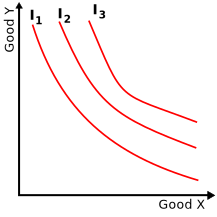
\includegraphics[width=0.7\linewidth]{./../images/Simple-indifference-curves} 

}

\caption{An example of an indifference map with three indifference curves represented.}\label{fig:indifference-curve1}
\end{figure}

\begin{figure}

{\centering \includegraphics[width=0.7\linewidth]{./../images/Indifference-curves-perfect-substitutes} 

}

\caption{Three indifference curves where Goods X and Y are perfect substitutes. The gray line perpendicular to all curves indicates the curves are mutually parallel.}\label{fig:indifference-curve2}
\end{figure}

\begin{figure}

{\centering \includegraphics[width=0.7\linewidth]{./../images/Indifference-curves-perfect-complements} 

}

\caption{Indifference curves for perfect complements X and Y. The elbows of the curves are collinear.}\label{fig:indifference-curve3}
\end{figure}

In Figure \ref{fig:indifference-curve1}, the consumer would rather be on
I3 than I2, and would rather be on I2 than I1, but does not care where
he/she is on a given indifference curve. The slope of an indifference
curve (in absolute value), known by economists as the marginal rate of
substitution, shows the rate at which consumers are willing to give up
one good in exchange for more of the other good. For most goods the
marginal rate of substitution is not constant so their indifference
curves are curved. The curves are convex to the origin, describing the
negative substitution effect. As price rises for a fixed money income,
the consumer seeks the less expensive substitute at a lower indifference
curve. The substitution effect is reinforced through the income effect
of lower real income (Beattie-LaFrance). The negative slope of the
indifference curve incorporates the willingness of the consumer to make
trade offs.

If two goods are perfect substitutes then the indifference curves will
have a constant slope since the consumer would be willing to switch
between at a fixed ratio; shown in Figure \ref{fig:indifference-curve2}.
The marginal rate of substitution between perfect substitutes is
likewise constant.

If two goods are perfect complements then the indifference curves will
be L-shaped; shown in Figure \ref{fig:indifference-curve3}. Examples of
perfect complements include left shoes compared to right shoes: the
consumer is no better off having several right shoes if she has only one
left shoe - additional right shoes have zero marginal utility without
more left shoes, so bundles of goods differing only in the number of
right shoes they include - however many - are equally preferred. The
marginal rate of substitution is either zero or infinite.

The different shapes of the curves imply different responses to a change
in price as shown from demand analysis in consumer theory. The results
will only be stated here. A price-budget-line change that kept a
consumer in equilibrium on the same indifference curve:

\begin{itemize}
\item
  in Figure \ref{fig:indifference-curve1} would reduce quantity demanded
  of a good smoothly as price rose relatively for that good.
\item
  in Figure \ref{fig:indifference-curve2} would have either no effect on
  quantity demanded of either good (at one end of the budget constraint)
  or would change quantity demanded from one end of the budget
  constraint to the other.
\item
  in Figure \ref{fig:indifference-curve3} would have no effect on
  equilibrium quantities demanded, since the budget line would rotate
  around the corner of the indifference curve.
\end{itemize}

\begin{figure}

{\centering 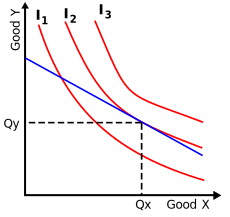
\includegraphics[width=0.7\linewidth]{./../images/Indifference_curves_showing_budget_line} 

}

\caption{Indifference curves and deduction of demand schedule for a simple good. To maximise utility, a household should consume at (Qx, Qy). Assuming it does, a full demand schedule can be deduced as the price of one good fluctuates.}\label{fig:expansion-path}
\end{figure}

\section{The law of diminishing marginal
utility}\label{the-law-of-diminishing-marginal-utility}

As an example, in a hot day, you drink water and as the consumption of
water increases marginal utility decreases. Each additional unit
consumed gives the consumer less additional utility than the one before.
This does not mean that total utility declines; four is better than
three, more is better than less. However, more is better than less at a
declining rate. At some point, the consumer can consume too much of a
good: water becomes a noneconomic good at the point when its marginal
utility becomes negative.

The Law of Diminishing Marginal Utility is used to show that if a
consumer has many pairs of pants (point A: 6 pairs of pants, 1 shirt),
she is willing to trade 3 pairs of pants for one additional shirt (point
B: 3 pairs of pants, 2 shirts). On the other hand, if the consumer had 5
shirts and only one pair of pants (point C), she would be willing to
give up two shirts for the second pair of pants (point D: 2 pairs of
pants and 3 shirts). A consumer's willingness to trade one good for
another depends on how much of each good he or she has. The first unit
provides the higher level of satisfaction, and consumption of subsequent
units provide less additional utility, as shown in Figure
\ref{fig:dim-mar-utility}.

\begin{figure}

{\centering \includegraphics[width=0.9\linewidth]{Farm_Management_and_Economics_files/figure-latex/dim-mar-utility-1} 

}

\caption{Law of diminishing marginal utility}\label{fig:dim-mar-utility}
\end{figure}

\begin{quote}
\emph{``Will you ever trade diamond for water? Yes!''} --- The
Diamond-Water paradox
\end{quote}

Law of Diminishing Marginal Utility: \newline Marginal utility declines
as more of a good or service is consumed during a given time period.

The law of diminishing marginal utility implies that consumers will not
spend all of their income on one good, because the marginal utility of
continuing to buy the same good declines. Instead, consumers use their
money to buy a variety of goods.

\section{Price and income effects}\label{price-and-income-effects}

\section{Law of Demand}\label{law-of-demand}

\subsection{Demand}\label{demand}

``Demand'' and ``supply'' are the twin driving forces of the market
economy. Demand is not just about measuring what people want; for
economists, it refers to the amount of a good or service that people are
both willing and able to buy. The demand curve measures the relationship
between the price of a good and the amount of it demanded. Usually, as
the price rises, fewer people are willing and able to buy it; in other
words, demand falls (but see giffen goods, normal goods and inferior
goods). When demand changes, economists explain this in one of two ways.
A movement along the demand curve occurs when a price change alters the
quantity demanded; but if the price were to go back to where it was
before, so would the amount demanded. A shift in the demand curve occurs
when the amount demanded would be different from what it was previously
at any chosen price, for example, if there is no change in the market
price, but demand rises or falls. The slope of the demand curve
indicates the \textbf{elasticity of demand}.

Policymakers seek to manipulate aggregate demand to keep the economy
growing as fast as is possible without pushing up inflation. Keynesians
try to manage demand through fiscal policy; monetarists prefer to use
the money supply. Neither approach has been especially successful in
practice, particularly when attempting to manage short-term demand
through fine tuning.

\textbf{Demand curve}

A graph showing the relationship between the price of a good and the
amount of demand for it at different prices.

\begin{figure}

{\centering \includegraphics[width=1.05\linewidth]{Farm_Management_and_Economics_files/figure-latex/demand-curve1-1} 

}

\caption{Demand and supply curves showing change in demand}\label{fig:demand-curve1}
\end{figure}

\section{Law of Supply}\label{law-of-supply}

\subsection{Supply}\label{supply}

\section{Economics of production}\label{economics-of-production}

It describes the physical relationship between inputs and outputs, and
describes the economics of transforming inputs into products; resources
into goods.

\subsection{The production function}\label{the-production-function}

The production of goods and services is a logical place to begin
studying the economics of agricultural production. During the production
process, firms, or producers, combine inputs into outputs for sale to
consumers. The process can be quite complex. Then follows the production
activities undertaken by firms. The discussion then shifts to the
behavior of consumers, or households. All of this leads to consideration
of the interactions of consumers and producers in markets.
\textbf{Production} is the process of producing goods and services. This
process requires scarce resources.

Inputs have several different names: Inputs = factors = factors of
production = resources = A, L, K, M

\begin{quote}
\textbf{A}: Land (Natural and biological resources, climate.)
\newline \textbf{L}: Labor (Human resources.) \newline \textbf{K}:
Capital (Manufactured resources, which include buildings, machines,
tools, and equipment.) \newline \textbf{M}: Management (The
entrepreneur, or individual, who combines the other resources into
inputs.)
\end{quote}

\subsection{Economic concept of time
periods}\label{economic-concept-of-time-periods}

In economics, these terms have specific meanings, but not meanings
related to a specific length of time such as minutes, days, or weeks.
The length of the long run, the short run, and the immediate run depend
on the specific situation.

The \textbf{Immediate Run} is a period of time during which all of the
inputs available to a producer are fixed and cannot be changed. The
producer cannot change the quantity of any input. A wheat producer
purchases land, labor, seed, machinery, fertilizer, and chemicals. After
the planting season, the producer is unlikely to be able to alter or use
either more or less of the quantity of these inputs to affect the
progress of the crop. This situation defines the immediate run.

As time passes, the producer will have more flexibility to change the
quantities of inputs. In a three-month period, this producer is able to
alter the number of hours of work hired, but cannot change the number of
acres of land that are in production or, after a certain period, add
more fertilizer. This situation is called the \textbf{Short Run} ,
defined as a period when some inputs are fixed (the quantities of inputs
used cannot be altered) and some inputs are variable (the quantities of
inputs can be changed).

The quantities of some agricultural inputs are not easy to change in the
short run. Land is a common example. Most producers cannot acquire more
land in a short length of time. Therefore, the acres of land available
to one producer remain fixed in the Short Run (SR). Similarly, machinery
and equipment (combines, tractors, and plows) are very expensive, and
many producers cannot rapidly increase or decrease the number of these
inputs. During that period when a farmer is unable to alter the quantity
of inputs, the inputs are fixed, and the farmer is in the Short Run
(SR). However, in the short run, some inputs are variable. For example,
the producer could alter the level of chemicals, fertilizer, labor, or
management. In the \textbf{Long Run} (LR), all inputs are variable.

Over long run, producer may buy or sell machinery or land. They can also
adjust the size of their farm. the long run is however long it takes to
adjust the levels of inputs. This differs from farm to farm and from
business to business.

\subsection{Inputs}\label{inputs}

\(\textbf{Fixed input}\) = An input whose quantity does not vary with
the level of output.

\(\textbf{Variable input}\) = An input that when changed affects the
level of output.

\subsection{Physical production
relationships}\label{physical-production-relationships}

Understanding the production function requires discussion of
transforming inputs into outputs. Suppose a wheat farmer in Bhairahawa
uses capital, labor, land, and management to produce corn. Recall the
generalized production function for his farming activity:

\[Y = f(L, K, A, M)\]

Understanding the impact of labor on corn output requires holding the
levels of all other inputs constant.

\[Y = f(L|K, A, M)\]

This leads to an understanding of production efficiency, explained in
the next section.

\subsubsection{Constant, increasing, decreasing, and negative
returns}\label{constant-increasing-decreasing-and-negative-returns}

The level of inputs as reported in the production function determines
the level of output (the production function describes the physical
relationship between inputs and output). The production process can take
on different forms: Constant Returns, Increasing Returns, Decreasing
Returns, and Negative Returns . The word \emph{returns} refers to
changes in output that occur as quantities of inputs increase
incrementally. Think of increasing the level of inputs by one unit at a
time, and measuring how output responds to each change. This incremental
way of approaching a problem is one cornerstone of ``\textbf{thinking
like an economist.}'' In a production process characterized by Constant
Returns , each additional unit of input is equally as productive as all
other units of input.

\textbf{Constant Returns}: When each additional unit of input added to
the production process yields a constant level of output relative to the
previous unit of input. Output increases at a constant rate. Table
\ref{tab:constant-returns} and Figure \ref{fig:constant-returns1} show
physical production relationship with constant rate of returns.

\begin{table}

\caption{\label{tab:constant-returns}Physical production relationship: constant rate of returns}
\begin{tabular}[t]{>{\centering\arraybackslash}p{10em}>{\centering\arraybackslash}p{10em}>{\centering\arraybackslash}p{10em}}
\toprule
Y (Output; wheat yield) & X (Inputs; planting density) & Added output $ \newline (\delta Y/ \delta X)$\\
\midrule
0 & 0 & \bgroup\fontsize{12}{14}\selectfont \textcolor[HTML]{BBBBBB}{\textbf{NA}}\egroup{}\\
1 & 1 & \bgroup\fontsize{12}{14}\selectfont \textcolor[HTML]{2A788E}{\textbf{1}}\egroup{}\\
2 & 2 & \bgroup\fontsize{12}{14}\selectfont \textcolor[HTML]{2A788E}{\textbf{1}}\egroup{}\\
3 & 3 & \bgroup\fontsize{12}{14}\selectfont \textcolor[HTML]{2A788E}{\textbf{1}}\egroup{}\\
4 & 4 & \bgroup\fontsize{12}{14}\selectfont \textcolor[HTML]{2A788E}{\textbf{1}}\egroup{}\\
5 & 5 & \bgroup\fontsize{12}{14}\selectfont \textcolor[HTML]{2A788E}{\textbf{1}}\egroup{}\\
\bottomrule
\end{tabular}
\end{table}

\begin{figure}

{\centering \includegraphics[width=0.9\linewidth]{Farm_Management_and_Economics_files/figure-latex/constant-returns1-1} 

}

\caption{Wheat yield: constant returns}\label{fig:constant-returns1}
\end{figure}

\textbf{Increasing Returns}: When each additional unit of input added to
the production process yields an increasing level of output relative to
the previous unit of input. Output increases at an increasing rate.
Table \ref{tab:increasing-returns} and Figure
\ref{fig:increasing-returns1} show physical production relationship with
increasing rate of returns.

\textbf{Decreasing Returns}: When each additional unit of input added to
the production process yields less additional output relative to the
previous unit of input. Output increases at a decreasing rate. Table
\ref{tab:decreasing-returns} and Figure \ref{fig:decreasing-returns1}
show physical production relationship with decreasing rate of returns.

\textbf{Negative Returns}: When each additional unit of input added to
the production process results in lower total output relative to the
previous unit of input. Output decreases. Table
\ref{tab:negative-returns} and Figure \ref{fig:negative-returns1} show
physical production relationship with negative rate of returns.

\begin{table}

\caption{\label{tab:increasing-returns}Physical production relationship: increasing rate of returns}
\begin{tabular}[t]{>{\centering\arraybackslash}p{10em}>{\centering\arraybackslash}p{10em}>{\centering\arraybackslash}p{10em}}
\toprule
Y (Output; wheat yield) & X (Inputs; planting density) & Added output $ \newline (\delta Y/ \delta X)$\\
\midrule
0 & 0 & \bgroup\fontsize{12}{14}\selectfont \textcolor[HTML]{BBBBBB}{\textbf{NA}}\egroup{}\\
10 & 1 & \bgroup\fontsize{8}{10}\selectfont \textcolor[HTML]{440154}{\textbf{10}}\egroup{}\\
30 & 2 & \bgroup\fontsize{10}{12}\selectfont \textcolor[HTML]{414487}{\textbf{20}}\egroup{}\\
60 & 3 & \bgroup\fontsize{12}{14}\selectfont \textcolor[HTML]{2A788E}{\textbf{30}}\egroup{}\\
100 & 4 & \bgroup\fontsize{14}{16}\selectfont \textcolor[HTML]{22A884}{\textbf{40}}\egroup{}\\
150 & 5 & \bgroup\fontsize{16}{18}\selectfont \textcolor[HTML]{7AD151}{\textbf{50}}\egroup{}\\
\bottomrule
\end{tabular}
\end{table}

\begin{figure}

{\centering \includegraphics[width=0.9\linewidth]{Farm_Management_and_Economics_files/figure-latex/increasing-returns1-1} 

}

\caption{Wheat yield: increasing returns}\label{fig:increasing-returns1}
\end{figure}

\begin{table}

\caption{\label{tab:decreasing-returns}Physical production relationship: decreasing rate of returns}
\begin{tabular}[t]{>{\centering\arraybackslash}p{10em}>{\centering\arraybackslash}p{10em}>{\centering\arraybackslash}p{10em}}
\toprule
Y (Output; wheat yield) & X (Inputs; planting density) & Added output $ \newline (\delta Y/ \delta X)$\\
\midrule
0 & 0 & \bgroup\fontsize{12}{14}\selectfont \textcolor[HTML]{BBBBBB}{\textbf{NA}}\egroup{}\\
10 & 1 & \bgroup\fontsize{16}{18}\selectfont \textcolor[HTML]{7AD151}{\textbf{10}}\egroup{}\\
18 & 2 & \bgroup\fontsize{14}{16}\selectfont \textcolor[HTML]{22A884}{\textbf{8}}\egroup{}\\
24 & 3 & \bgroup\fontsize{12}{14}\selectfont \textcolor[HTML]{2A788E}{\textbf{6}}\egroup{}\\
28 & 4 & \bgroup\fontsize{10}{12}\selectfont \textcolor[HTML]{414487}{\textbf{4}}\egroup{}\\
30 & 5 & \bgroup\fontsize{8}{10}\selectfont \textcolor[HTML]{440154}{\textbf{2}}\egroup{}\\
\bottomrule
\end{tabular}
\end{table}

\begin{figure}

{\centering \includegraphics[width=0.9\linewidth]{Farm_Management_and_Economics_files/figure-latex/decreasing-returns1-1} 

}

\caption{Wheat yield: decreasing returns}\label{fig:decreasing-returns1}
\end{figure}

\begin{table}

\caption{\label{tab:negative-returns}Physical production relationship: negative rate of returns}
\begin{tabular}[t]{>{\centering\arraybackslash}p{10em}>{\centering\arraybackslash}p{10em}>{\centering\arraybackslash}p{10em}}
\toprule
Y (Output; wheat yield) & X (Inputs; planting density) & Added output $ \newline (\delta Y/ \delta X)$\\
\midrule
0 & 0 & \bgroup\fontsize{12}{14}\selectfont \textcolor[HTML]{BBBBBB}{\textbf{NA}}\egroup{}\\
10 & 1 & \bgroup\fontsize{16}{18}\selectfont \textcolor[HTML]{7AD151}{\textbf{10}}\egroup{}\\
9 & 2 & \bgroup\fontsize{9}{11}\selectfont \textcolor[HTML]{472C7A}{\textbf{-1}}\egroup{}\\
7 & 3 & \bgroup\fontsize{9}{11}\selectfont \textcolor[HTML]{48186A}{\textbf{-2}}\egroup{}\\
4 & 4 & \bgroup\fontsize{8}{10}\selectfont \textcolor[HTML]{440154}{\textbf{-3}}\egroup{}\\
1 & 5 & \bgroup\fontsize{8}{10}\selectfont \textcolor[HTML]{440154}{\textbf{-3}}\egroup{}\\
\bottomrule
\end{tabular}
\end{table}

\begin{figure}

{\centering \includegraphics[width=0.9\linewidth]{Farm_Management_and_Economics_files/figure-latex/negative-returns1-1} 

}

\caption{Wheat yield: negative returns}\label{fig:negative-returns1}
\end{figure}

\section{Productivity}\label{productivity}

The relationship between inputs and output, which can be applied to
individual factors of production or collectively. Labour productivity is
the most widely used measure and is usually calculated by dividing total
output by the number of workers or the number of hours worked. Total
factor productivity attempts to measure the overall productivity of the
inputs used by a firm or a country.

Alas, the usefulness of productivity statistics is questionable. The
quality of different inputs can change significantly over time. There
can also be significant differences in the mix of inputs. Furthermore,
firms and countries may use different definitions of their inputs,
especially capital. That said, much of the difference in countries'
living standards reflects differences in their productivity. Usually,
the higher their productivity is the better, but this is not always so.
In the UK during the 1980s, labour productivity rose sharply, leading
some economists to talk of a ``productivity miracle''. Others disagreed,
saying that productivity had risen because unemployment had risen - in
other words, the least productive workers had been removed from the
figures on which the average was calculated.

There was a similar debate in the United States starting in the late
1990s. Initially, economists doubted that a productivity miracle was
taking place. But by 2003, they conceded that during the previous five
years the United States enjoyed the fastest productivity growth in any
such period since the second world war. Over the whole period from 1995,
labour productivity growth averaged almost 3\% a year, twice the average
rate over the previous two decades. That did not stop economists
debating why the miracle had occurred.

\section{Yield}\label{yield}

The annual income from a security, expressed as a percentage of the
current market price of the security. The yield on a share is its
dividend divided by its price. A bond yield is also known as its
interest rate: the annual coupon divided by the market price.

Yield curve is a shorthand for comparisons of the interest rate on
government bonds of different maturity. If investors think it is riskier
to buy a bond with 15 years until it matures than a bond with five years
of life, they will demand a higher interest rate (yield) on the
longer-dated bond. If so, the yield curve will slope upwards from left
(the shorter maturities) to right. It is normal for the yield curve to
be positive (upward sloping, left to right) simply because investors
normally demand compensation for the added risk of holding longer-term
securities. Historically, a downward-sloping (or inverted) yield curve
has been an indicator of recession on the horizon, or, at least, that
investors expect the central bank to cut short-term interest rates in
the near future. A flat yield curve means that investors are indifferent
to maturity risk, but this is unusual. When the yield curve as a whole
moves higher, it means that investors are more worried that inflation
will rise for the foreseeable future and therefore that higher interest
rates will be needed. When the whole curve moves lower, it means that
investors have a rosier inflationary outlook.

Even if the direction (up or down) of a yield curve is unchanged, useful
information can be gleaned from changes in the spreads between yields on
bonds of different maturities and on different sorts of bonds with the
same maturity (such as government bonds versus corporate bonds, or
thinly traded bonds versus highly liquid bonds).

Comparing the performance of bonds and shares is done through
\textbf{yield gap}. The gap is defined as the average yield on equities
minus the average yield on bonds. Because shares are usually riskier
investments than bonds, you might expect them to have a higher yield. In
practice, the yield gap is often negative, with bonds yielding more than
equities. This is not because investors regard equities as safer than
bonds (see equity risk premium). Rather, it is that they expect most of
the benefit from buying shares to come from an increase in their price
(capital appreciation) rather than from dividend payments. Bond
investors usually expect more of their gains to come from coupon
payments. They also worry that inflation will erode the real value of
future coupons, making them value current payments more highly than
those due in years to come. Moreover, the usefulness of the dividend
yield as a guide to the performance of shares has declined since the
early 1990s, as increasingly companies have chosen to return cash to
shareholders by buying back their own shares rather than paying out
bigger dividends.

\section{Marginal concept of cost and
revenue}\label{marginal-concept-of-cost-and-revenue}

The difference made by one extra unit of something. Marginal revenue is
the extra revenue earned by selling one more unit of something. The
marginal price is how much extra a consumer must pay to buy one extra
unit. Marginal utility is how much extra utility a person gets from
consuming (or doing) an extra unit of something. The marginal product of
labour is how much extra output a firm would get by employing an extra
worker, or by getting an existing worker to put in an extra hour on the
job. The marginal propensity to consume (or to save) measures by how
much a household's consumption (savings) would increase if its income
rose by, say, \$1. The marginal tax rate measures how much extra tax you
would have to pay if you earned an extra dollar. The marginal cost (or
whatever) can be very different from the average cost (or whatever),
which simply divides total costs (or whatever) by the total number of
units produced (or whatever). A common finding in microeconomics is that
small incremental changes can matter enormously. In general, thinking
``at the margin'' often leads to better economic decision-making than
thinking about the averages. Alfred marshall, the father of
neo-classical economics, based many of his theories of economic
behaviour on marginal rather than average behaviour. For instance,
givencertain plausible assumptions, a profit-maximising firm will
increase production up to the point where marginal revenue equals
marginal cost. This is because if marginal revenue exceeded marginal
cost, the firm could increase its profit by producing an extra unit of
output. Alternatively, if marginal cost exceeded marginal revenue, the
firm could increase its profit by producing fewer units of output. In
all walks of life, a basic rule of rational economic decision-making is:
do something only if the marginal utility you get from it exceeds the
marginal cost of doing it.

\section{Price}\label{price}

In equilibrium, what balances supply and demand. The price charged for
something depends on the tastes, income and elasticity of demand of
customers. It depends on the amount of competition in the market. Under
perfect competition, all firms are price takers. Where there is a
monopoly, or firms have some market power, the seller has some control
over the price, which will probably be higher than in a perfectly
competitive market. By how much more will depend on how much market
power there is, and on whether the firm(s) with the market power are
committed to profit maximisation. In some cases, firms may charge less
than the profit-maximising price for strategic or other reasons (called
predatory pricing).

\section{Diminishing returns}\label{diminishing-returns}

The more you have, the smaller is the extra benefit you get from having
even more; also known as diseconomies of scale (see economies of scale).
For instance, when workers have a lot of capital giving them a little
more may not increase their productivity anywhere near as much as would
giving the same amount to workers who currently have little or no
capital. This underpins the catch-up effect, whereby there is
(supposedly) convergence between the rates of growth of developing
countries and developed ones. In the new economy, some economists argue,
capital may not suffer from diminishing returns, or at least the amount
of diminishing will be much smaller. There may even be ever increasing
returns.

\section{Factors of production}\label{factors-of-production}

\textbf{Capital}

Money or assets put to economic use, the life-blood of capitalism.
Economists describe capital as one of the four essential ingredients of
economic activity, the factors of production, along with land, labour
and enterprise. Production processes that use a lot of capital relative
to labour are capital intensive; those that use comparatively little
capital are labour intensive. Capital takes different forms. A firm's
assets are known as its capital, which may include fixed capital
(machinery, buildings, and so on) and working capital (stocks of raw
materials and part-finished products, as well as money, that are used up
quickly in the production process). Financial capital includes money,
bonds and shares. human capital is the economic wealth or potential
contained in a person, some of it endowed at birth, the rest the product
of training and education, if only in the university of life. The
invisible glue of relationships and institutions that holds an economy
together is its social capital.

\textbf{Land}

One of the factors of production, along with labour, capital and
enterprise. Pending colonisation of the moon, it is in fairly fixed
supply. Marginal increases are possible by reclaiming land from the sea
and cutting down forests (which may impose large economic costs by
damaging the environment), but the expansion of deserts may slightly
reduce the amount of usable land. Owners earn money from land by
charging rent.

\textbf{Labor}

One of the factors of production, with land, capital and enterprise.
Among the things that determine the supply of labour are the number of
able people in the population, their willingness to work, labour laws
and regulations, and the health of the economy and firms. demand for
labour is also affected by the health of the economy and firms, labour
laws and regulations, as well as the price and supply of other factors
of production.

In a perfect market, wages (the price of labour) would be determined by
supply and demand. But the labour market is often far from perfect.
Wages can be less flexible than other prices; in particular, they rarely
fall even when demand for labour declines or supply increases. This wage
rigidity can be a cause of unemployment.

\textbf{Enterprise}

An entrepreneur is somebody who has the idea and enterprise to mix
together the other factors of production to produce something valuable.
An entrepreneur must be willing to take a risk in pursuit of a profit.

\section{Commodity}\label{commodity}

A comparatively homogeneous product that can typically be bought in
bulk. It usually refers to a raw material - oil, cotton, cocoa, silver -
but can also describe a manufactured product used to make other things,
for example, microchips used in personal computers. Commodities are
often traded on commodity exchanges. On average, the price of natural
commodities has fallen steadily in real terms in defiance of some
predictions that growing consumption of non-renewables such as copper
would force prices up. At times the oil price has risen sharply in real
terms, most notably during the 1970s, but this was caused not by the
exhaustion of limited supplies but by rationing by the opec cartel, or
war, or fear of it, particularly in the oil-rich Middle East.

\section{Market}\label{market}

\textbf{Competition}

The more competition there is, the more likely are firms to be efficient
and prices to be low. Economists have identified several different sorts
of competition. Perfect competition is the most competitive market
imaginable in which everybody is a price taker. Firms earn only normal
profits, the bare minimum profit necessary to keep them in business. If
firms earn more than this (excess profits), other firms will enter the
market and drive the price level down until there are only normal
profits to be made. Most markets exhibit some form of imperfect or
monopolistic competition. There are fewer firms than in a perfectly
competitive market and each can to some degree create barriers to entry.
So firms can earn some excess profits without a new entrant being able
to compete to bring prices down. The least competitive market is a
monopoly, dominated by a single firm that can earn substantial excess
profits by controlling either the amount of output in the market or the
price (but not both). In this sense it is a price setter. When there are
few firms in a market (oligopoly), they have the opportunity to behave
as a monopolist through some form of collusion (see cartel). A market
dominated by a single firm does not necessarily have monopoly power if
it is a contestable market. In such a market, a single firm can dominate
only if it produces as efficiently as possible and does not earn excess
profits. If it becomes inefficient or earns excess profits, another more
efficient or less profitable firm will enter the market and dominate it
instead.

\begin{enumerate}
\def\labelenumi{\arabic{enumi}.}
\tightlist
\item
  Perfect competition
\end{enumerate}

The most competitive market imaginable. Perfect competition is rare and
may not even exist. It is so competitive that any individual buyer or
seller has a negligible impact on the market price. Products are
homogeneous. information is perfect. Everybody is a price taker. firms
earn only normal profit, the bare minimum profit necessary to keep them
in business. If firms earn more than that (excess profits), the absence
of barriers to entry means that other firms will enter the market and
drive the price level down until there are only normal profits to be
made. Output will be maximised and price minimised. Contrast with
monopolistic competition, oligopoly and, above all, monopoly.

\begin{enumerate}
\def\labelenumi{\arabic{enumi}.}
\setcounter{enumi}{1}
\tightlist
\item
  Monopolistic competition
\end{enumerate}

Somewhere between perfect competition and monopoly, also known as
imperfect competition. It describes many real-world markets. Perfectly
competitive markets are extremely rare, and few firms enjoy a pure
monopoly; oligopoly is more common. In monopolistic competition, there
are fewer firms than in a perfectly competitive market and each can
differentiate its products from the rest somewhat, perhaps by
advertising or through small differences in design. These small
differences form barriers to entry. As a result, firms can earn some
excess profits, although not as much as a pure monopoly, without a new
entrant being able to reduce prices through competition. Prices are
higher and output lower than under perfect competition.

\begin{itemize}
\tightlist
\item
  Barriers to entry (or exit)

  \begin{itemize}
  \item
    How firms keep out competition - an important source of incumbent
    advantage. There are four main categories of barriers. They are:
  \item
    \begin{enumerate}
    \def\labelenumi{\arabic{enumi}.}
    \tightlist
    \item
      A firm may own a crucial resource, such as an oil well, or it may
      have an exclusive operating licence, for instance, to broadcast on
      a particular radio wavelength.
    \end{enumerate}
  \item
    \begin{enumerate}
    \def\labelenumi{\arabic{enumi}.}
    \setcounter{enumi}{1}
    \tightlist
    \item
      A big firm with economies of scale may have a significant
      competitive advantage because it can produce a large output at
      lower costs than can a smaller potential rival.
    \end{enumerate}
  \item
    \begin{enumerate}
    \def\labelenumi{\arabic{enumi}.}
    \setcounter{enumi}{2}
    \tightlist
    \item
      An incumbent firm may make it hard for a would-be entrant by
      incurring huge sunk costs, spending lots of money on things such
      as advertising, which any rival must match to compete effectively
      but which have no value if the attempt to compete should fail.
    \end{enumerate}
  \item
    \begin{enumerate}
    \def\labelenumi{\arabic{enumi}.}
    \setcounter{enumi}{3}
    \tightlist
    \item
      Powerful firms can discourage entry by raising exit costs, for
      example, by making it an industry norm to hire workers on
      long-term contracts, which make firing an expensive process.
    \end{enumerate}
  \end{itemize}
\end{itemize}

\begin{enumerate}
\def\labelenumi{\arabic{enumi}.}
\setcounter{enumi}{2}
\tightlist
\item
  Monopoly
\end{enumerate}

When the production of a good or service with no close substitutes is
carried out by a single firm with the market power to decide the price
of its output. Contrast with perfect competition, in which no single
firm can affect the price of what it produces. Typically, a monopoly
will produce less, at a higher price, than would be the case for the
entire market under perfect competition. It decides its price by
calculating the quantity of output at which its marginal revenue would
equal its marginal cost, and then sets whatever price would enable it to
sell exactly that quantity.

In practice, few monopolies are absolute, and their power to set prices
or limit supply is constrained by some actual or potential
near-competitors (see monopolistic competition). An extreme case of this
occurs when a single firm dominates a market but has no pricing power
because it is in a contestable market; that is, if it does not operate
efficiently, a more efficient rival firm will take its entire market
away. Antitrust policy can curb monopoly power by encouraging
competition or, when there is a natural monopoly and thus competition
would be inefficient, through regulation of prices. Furthermore, the
mere possibility of antitrust action may encourage a monopoly to
self-regulate its behaviour, simply to avoid the trouble an
investigation would bring.

\begin{enumerate}
\def\labelenumi{\arabic{enumi}.}
\setcounter{enumi}{3}
\tightlist
\item
  Oligopoly
\end{enumerate}

When a few firms dominate a market. Often they can together behave as if
they were a single monopoly, perhaps by forming a cartel. Or they may
collude informally, by preferring gentle non-price competition to a
bloody price war. Because what one firm can do depends on what the other
firms do, the behaviour of oligopolists is hard to predict. When they do
compete on price, they may produce as much and charge as little as if
they were in a market with perfect competition.

\textbf{Monopsony}

A market dominated by a single buyer. A monopsonist has the market power
to set the price of whatever it is buying (from raw materials to
labour). Under perfect competition, by contrast, no individual buyer is
big enough to affect the market price of anything.

\section{Diversification}\label{diversification}

Not putting all your eggs in one basket. Investors are encouraged to do
this by modern portfolio theory, as holding several different shares and
other assets helps to reduce risk. At the sharp end of business,
however, diversification is somewhat out of fashion. Economic studies of
diversifying corporate mergers have found that these often hurt the
shareholders of the acquiring firm; by contrast, diversified firms that
have sold off non-core businesses have typically made their shareholders
much better off.

\section{Equilibrium}\label{equilibrium}

When supply and demand are in balance. At the equilibrium price, the
quantity that buyers are willing to buy exactly matches the quantity
that sellers are willing to sell. So everybody is satisfied, unlike when
there is disequilibrium. In classical economics, it is assumed that
markets always tend towards equilibrium and return to it in the event
that something causes a temporary disequilibrium. general equilibrium is
when supply and demand are balanced simultaneously in all the markets in
an economy. keynes questioned whether the economy always moved to
equilibrium, for instance, to ensure full employment.

\section{GDP}\label{gdp}

Gross domestic product, a measure of economic activity in a country. It
is calculated by adding the total value of a country's annual output of
goods and services. GDP = private consumption + investment + public
spending + the change in inventories + (exports - imports). It is
usually valued at market prices; by subtracting indirect tax and adding
any government subsidy, however, GDP can be calculated at factor cost.
This measure more accurately reveals the income paid to factors of
production. Adding income earned by domestic residents from their
investments abroad, and subtracting income paid from the country to
investors abroad, gives the country's gross national product (GNP).

The effect of inflation can be eliminated by measuring GDP growth in
constant real prices. However, some economists argue that hitting a
nominal GDP target should be the main goal of macroeconomic policy. This
is because it would remind policymakers to take into account the effect
of their decisions on inflation, as well as on growth.

GDP can be calculated in three ways. The income method adds the income
of residents (individuals and firms) derived from the production of
goods and services. The output method adds the value of output from the
different sectors of the economy. The expenditure method totals spending
on goods and services produced by residents, before allowing for
depreciation and capital consumption. As one person's output is another
person's income, which in turn becomes expenditure, these three measures
ought to be identical. They rarely are because of statistical
imperfections. Furthermore, the output and income measures exclude
unreported economic activity that takes place in the black economy but
that may be captured by the expenditure measure.

GDP is disliked as an objective of economic policy by some because it is
not a perfect measure of welfare. It does not include aspects of the
good life such as some leisure activities. Nor does it include
economically valuable activities that are not paid for, such as parents
teaching their children to read. But it does include some things that
lower the quality of life, such as activities that damage the
environment.

\section{Balance of trade}\label{balance-of-trade}

The total of all the money coming into a country from abroad less all of
the money going out of the country during the same period. This is
usually broken down into the current account and the capital account.

The current account includes:

\begin{itemize}
\tightlist
\item
  Visible trade (known as merchandise trade in the United States), which
  is the value of exports and imports of physical goods;
\item
  Invisible trade, which is receipts and payments for services, such as
  banking or advertising, and other intangible goods, such as
  copyrights, as well as cross-border dividend and interest payments;
\item
  Private transfers, such as money sent home by expatriate workers;
\item
  Official transfers, such as international aid.
\end{itemize}

The capital account includes:

\begin{itemize}
\tightlist
\item
  Long-term capital flows, such as money invested in foreign firms, and
  profits made by selling those investments and bringing the money home;
\item
  Short-term capital flows, such as money invested in foreign currencies
  by international speculators, and funds moved around the world for
  business purposes by multinational companies. These short-term flows
  can lead to sharp movements in exchange rates, which bear little
  relation to what currencies should be worth judging by fundamental
  measures of value such as purchasing power parity.
\end{itemize}

As bills must be paid, ultimately a country's accounts must balance
(although because real life is never that neat a balancing item is
usually inserted to cover up the inconsistencies). ``Balance of payments
crisis'' is a politically charged phrase. But a country can often
sustain a current account deficit for many years without its economy
suffering, because any deficit is likely to be tiny compared with the
country's national income and wealth. Indeed, if the deficit is caused
by firms importing technology and other capital goods from abroad, which
will improve their productivity, the economy may benefit. A deficit that
has to be financed by the public sector may be more problematic,
particularly if the public sector faces limits on how much it can raise
taxes or borrow or has few financial reserves. For instance, when the
Russian government failed to pay the interest on its foreign debt in
August 1998 it found it impossible to borrow any more money in the
international financial markets. Nor was it able to increase taxes in
its collapsing economy or to find anybody within Russia willing to lend
it money. That truly was a balance of payments crisis.

In the early years of the 21st century, economists started to worry that
the United States would find itself in a balance of payments crisis. Its
current account deficit grew to over 5\% of its GDP, making its economy
increasingly reliant on foreign credit.

\section{Free trade}\label{free-trade}

The ability of people to undertake economic transactions with people in
other countries free from any restraints imposed by governments or other
regulators. Measured by the volume of imports and exports, world trade
has become increasingly free in the years since the second world war. A
fall in barriers to trade, as a result of the general agreement on
tariffs and trade and its successor, the world trade organisation, has
helped stimulate this growth. The volume of world merchandise trade at
the start of the 21st century was about 17 times what it was in 1950,
and the world's total output was not even six times as big. The ratio of
world exports to GDP had more than doubled since 1950. Of this, trade in
manufactured goods was worth three times the value of trade in services,
although the share of services trade was growing fast.

For economists, the benefits of free trade are explained by the theory
of comparative advantage, with each country doing those things in which
it is comparatively more efficient. As long as each country specialises
in products in which it has a comparative advantage, trade will be
mutually beneficial. Some critics of free trade argue that trade with
developing countries, where wages are usually lower and working hours
longer than in developed countries, is unfair and will wipe out jobs in
high-wage countries. They want autarky or fair trade.

Real-world trade patterns sometimes seem to challenge the theory of
comparative advantage. Most trade occurs between countries that do not
have huge cost differences. The biggest trading partner of the United
States, for instance, is Canada. Well over half the exports from France,
Germany and Italy go to other european union countries. Moreover, these
countries sell similar things to each other: cars made in France are
exported to Germany, and German cars go to France. The main reason seems
to be cross-border differences in consumer tastes. But the agricultural
exports of Australia, say, or Saudi Arabia's reliance on oil, do clearly
stem from their particular stock of natural resources. Also poorer
countries often have more unskilled labour, so they export simple
manufactures such as clothing.

\chapter{Farm management and
accounting}\label{farm-management-and-accounting}

\section{Farm management}\label{farm-management}

Farm management is a systems-related professional discipline which
relates to the description, construction, analysis and evaluation of
farm systems of farm-household systems (Order Level 12, as described
below). To a layman farm management probably means just that - a body of
activities and procedures carried out by a farmer in the ongoing
management of his or her farm and for which advice may be available from
professional specialists in farm management.

Farm management as carried out by farmers has been defined (Dillon 1980,
p.~258) as `the process by which resources and situations are
manipulated by the farm manager in trying, with less than full
information, to achieve his {[}or her{]} goals'.

\subsection{Meaning of Farm
management}\label{meaning-of-farm-management}

Farm management is the science (and art) of optimizing the use of
resources in the farm component of farm-households, and of achieving the
optimal functioning of these systems in relation to household-specified
objectives; and since Order farm-household systems consist structurally
of subsystems, farm management is also concerned with the operation of
subservient subsystems of lower levels (Order Levels below 9) in such
fashion as to optimize the whole-farm system. But when dealing with
small farms, that farm management extends also to the family or
household component, thus its true scope extends to Order Level 12
systems. Sometimes, upper order levels are also the necessary
considerations while making economic decisions.

It is also a very pertinent branch of economics as economics is the
science of making choices so as to best achieve desired objectives. It
comprises making rational choices, e.g., choice of which crops to grow
or to the choice between using an insecticide or using environmentally
friendly integrated pest management. Aside from this wide applicability
of economic analysis, financial analysis of farm, a subset of economic
analysis, is the natural way in which to economic analysis is conducted.
It is however restricted to matters that are of a financial or monetary
nature. In some cases it may be feasible to facilitate economic analysis
of possible choices by imputing money values to possible gains and
losses. And in yet other cases, such as assessing the resource
sustainability and environmental compatibility of alternative farm
systems, it may often be infeasible to impute money values to the gains
and losses of alternative choices. Decisions must then be made using
economic analysis based on non-money values, intuition and judgement.

\subsection{Characteristics/Features of Farm
management}\label{characteristicsfeatures-of-farm-management}

Features of farm mangement can be drawn from the structural elements
that comprise a farm-household system:

\begin{enumerate}
\def\labelenumi{\arabic{enumi}.}
\item
  Boundaries: The boundaries of the farm-household system set it apart
  from other systems and from the world at large. These boundaries are
  provided partly by the structural characteristics of the particular
  \emph{type of farm} (small subsistence, small independent, large,
  commercial, \ldots{}), and partly by the purpose of analysis, i.e., to
  some extent they are subjective and relate to more than the simple
  physical boundary of the farm.
\item
  Household: The household plays two roles: first, it provides purpose
  and management to its associated farm system and, second, it is the
  major beneficiary of its associated farm system. In its first role it
  provides purpose, operating objectives and management to the farm
  component of the farm-household system according to its broad domestic
  and social goals. Obviously these goals vary widely with culture,
  tradition and the degree of commercialisation and external influences
  to which the household is exposed. However, one would probably be not
  too far wrong in offering a generalization that the primary economic
  goal on most small farms is security and the primary non-economic goal
  is social acceptance (Clayton 1983). If this is correct, the primary
  objectives for the farm are, first, production of a low-risk
  sustainable subsistence for primary system beneficiaries; second,
  generation of a cash income to meet needs not directly met in the form
  of food and other farm-produced materials; and third, pursuit of both
  of these in ways which are not in conflict with local culture and
  tradition.
\item
  Operating plan: The above objectives are pursued through preparation
  and execution of a farm operating plan. The core of this may be taken
  as selection of the best possible mix of agro-technical processes,
  activities, enterprises and fixed capital.
\item
  Production-enabling resources: The resource pool
\item
  Final product-generating enterprises
\item
  Resource-generating activities: They are intended to supplement or
  entirely supply the resource pool
\item
  Agro-technical processes: These are defined as systems of Order Levels
  1 and 2. Processes may be of a biological or mechanical kind. They are
  a shorthand designation of all the potentially complex and
  interrelated physical and biological factors underlying production
  from crop or livestock species, only some of which may be economically
  relevant.
\item
  Whole-farm service matrix: consists of fixed farm capital which
  provides a flow of services to all other elements of the system,
  particularly to Elements 5, 6 and 7 but it is not specific to any one
  of them.
\item
  Structural (interdependence) coefficients
\item
  Time dimension.
\end{enumerate}

The other broader relevant features of farm management are:

\begin{enumerate}
\def\labelenumi{\arabic{enumi}.}
\item
  Practical science It is the practical science because concepts of farm
  management imparts farmer the knowledge regarding choices and economic
  decision making process of crop production, livestock production, and
  enterprise integration. It includes enabling farmer to adequately
  consider his/her condition -- Availability of resources, factors of
  production such as land, soil and environmental status that determine
  the productivity, volume and schedule of work, distribution of family
  labor, financial necessities, etc.
\item
  Profit oriented Farm management aims at maximization of return or
  profit on investment. Although the scale at which profit can be
  derived depends on several factors such as nature of enterprise
  (whether it is more risk prone or extractive, or is it more
  precautionary). A floriculture business seeks prolong the storage and
  production of cut-flowers. As well as, in the first place, it seeks a
  more profitable market where potential customers have higher buying
  capacity for the flower product.
\item
  Integration of science The FM has far-reaching/wide integration to
  other fields of sciences. Basic facts and information of applied
  sciences, i.e., Horticulture, agronomy, plant protection, animal
  husbandry, soil science have special place in running a farm
  enterprise. Mainly, technical efficiency and problem
  solving/enterpreneurial skills are acquired through subject matter
  expertise.
\item
  Micro approach It has a mico approach to management of farm units. A
  farm household on the whole is a single unit of management. Testing of
  and recommendations for resource are based on the farm status and
  suitability. With regard to availability of resources, opportunities
  that arise and the problem needed to be tackled, each farm is unique
  and therefore requires a micro-economic approach to management.
\item
  Broader field Although concepts of micro-economics have high relevance
  to FM, it integrates principles and practices of several disciplines
  in the real life scenario. Since it appreciates knowledge from many
  other fields of sciences, farm management specialist has to be a good
  learner and a broad practitioner. Thus the branch of economics suits
  ``Jack of many trades and Master of one'' principle.
\item
  Farm unit as a whole Individual farm is the unit of decision making,
  and the unit that has widest implication of the decision. Similarly,
  the farm resources availablity status of the farm that is being
  managed influence the most on planning and decision making process of
  the farm. When integrated systems are of concern, optimization of
  whole farm rather than a single enterprise is sought.
\end{enumerate}

\subsection{Farming system order
level}\label{farming-system-order-level}

Meaning of farm management can be clearly derived from the
\textbf{farming system order level} description (shown in Figure
\ref{fig:fs-order-level}).

\begin{figure}

{\centering \includegraphics[width=1\linewidth]{./../images/Farming_system_levels} 

}

\caption{Farming system order levels}\label{fig:fs-order-level}
\end{figure}

\begin{itemize}
\item
  Order Level 1: Uni-dimensional process systems. Systems of this lowest
  order are of an agro-technical nature. They involve an issue or
  problem which for purposes of analysis or management is abstracted
  from the context in which it naturally or normally occurs. One example
  is the application of a single fertilizer element, say nitrogen (N),
  to a crop and consequent plant response to N in terms of crop yield Y.
  As noted previously, systems of this order are primarily the domain of
  physical scientists, but those systems which have practical relevance
  for farmers thereby also have an economic dimension and so fall within
  the scope of farm economics. Such simple single-dimensional systems
  are examined as processes and as input-output response relationships.
\item
  Order Level 2: Multi-dimensional process systems. Systems of this
  second order are also concerned with limited agro-technical
  relationships and again they are primarily the domain of physical
  scientists. They differ from Order Level 1 systems in that they take -
  or are defined to take - a wider and more realistic view of a subject
  or problem. To use the same example of fertilizer response: at Order
  Level 2 an agro-technical system might involve the response of plant
  growth or yield Y to not one but to several or a large number of input
  factors such as nitrogen, phosphorous, irrigation water, crop hygiene,
  soil tilth etc. These multi-dimensional systems too are examined as
  processes and as response relationships. Order Level 2 systems can be
  viewed as aggregations (often interactive) of constituent Order Level
  1 systems.
\item
  Order Level 3: Enabling-activity systems. Systems of this order are
  certain enabling activities which generate an intermediate product
  intended for use as an input/resource by enterprises which do produce
  a final product. An example is offered by a legume crop turned under
  to provide fertility for a following (final product-generating) paddy
  crop. There will often be alternative ways of obtaining this resource:
  e.g., stripping leaves off leguminous trees, keeping cattle for their
  manure, or buying a bag of fertilizer. These are all enabling,
  resource-generating activities but only some of them, the complex
  ones, warrant designation as systems. They are intended to supply
  resources to systems of Order Levels 4 and 6.
\item
  Order Level 4: Crop systems. Systems of this order relate to the
  production of individual crops; but if these are primarily intended to
  produce inputs for other crops or livestock, they are regarded as
  systems of Order Level 3. On many small farms, crop and livestock
  enterprises produce both final products and resources.
\item
  Order Level 5: All crop systems. Systems of this order, known also as
  cropping systems, refer to the combined system of all the individual
  crops on a farm. On a farm with a single mono-crop, this Order Level 5
  system will obviously be equivalent to an Order Level 3 system; but on
  small mixed farms there will usually be four, five, six or more
  different crops (of Order Levels 3 and 4) grown in some degree of
  combination and as many as 20 or more on the highly diversified
  forest-garden farms of South Asia.
\item
  Order Level 6: Animal systems. These systems relate to single-species
  animal enterprises or activities - e.g., dairy cows, camels, fish,
  ducks. They are the animal equivalent of Order Level 4 (i.e.,
  individual crop) systems.
\item
  Order Level 7: All animal systems. These systems are the aggregation
  of all Order Level 6 (sub)systems on a farm. Known as livestock
  systems, they are the animal equivalent of Order Level 5 (i.e., all
  crop) systems.
\item
  Order Level 8: Resource pool. This subsystem is a conceptual device
  for farm-system planning in which resources and fixed-capital services
  required by other subsystems are `stored' in a `resource pool' from
  which they are allocated to the other subsystems (of Order Levels 1,
  2, 3, 4 and 6). The resource pool is central to operation of the whole
  farm-household system.
\item
  Order Level 9: Farm service matrix. A system of this Order Level
  consists of all the fixed capital resources of a farm which are
  pertinent to the operation of the farm as a whole but are not assigned
  to the exclusive use of any particular enterprise or activity: land,
  fences, barns, irrigation channels and work oxen are common examples.
  Some of these capital items are true (sub)systems, having
  interdependence among their component parts (as in an irrigation
  storage/delivery/distribution network, a grain drying facility, an
  integrated network of soil conservation structures etc.). Some are
  only things (e.g., fences, a plough, a barn). But, in its totality,
  such capital is managed and manipulated as a system for the purpose of
  providing general services which, while not specific to them, enable
  the functioning of lower Order Level systems of the farm.
\item
  Order Level 10: Whole-farm systems. Systems of this Order Level
  consist of all the lower Order Level (sub)systems which go to make up
  a farm. They consolidate in a single entity all the farm fixed
  capital, all the operating capital, all the final-product enterprises,
  all the activities and all the agro-technical processes which underlie
  such enterprises and activities. Structuring and managing systems of
  this Order Level are the main tasks or focus of farm management as
  carried out, on the one hand, by farmers and as investigated, on the
  other hand, by farm management economists in their professional
  capacity of providing advice to farm managers, development agencies
  and governments.\newline The terms \emph{farm system} and
  \emph{farming system} are often used interchangeably. The practice is
  to use farm system to refer to the structure of an individual farm,
  and farming system to refer to broadly similar farm types in specific
  geographical areas or recommendation domains, e.g., the wet paddy
  farming system of West Java or the grain-livestock farming systems of
  Sind.
\item
  Order Level 11: Household systems. On small farms the household itself
  is the most dynamic and complex of all farm-level systems, although it
  is a social system not an agricultural one. It dominates the
  agricultural systems which comprise the farm component. It has two
  functions: as household it provides purpose and management to the farm
  component, and as major system beneficiary it receives and allocates
  system outputs to itself and other beneficiaries.
\item
  Order Level 12: Farm-household systems. These consist of two
  components or (sub)systems of Order Levels 10 and 11, i.e., the
  whole-farm system and its associated household system, respectively.
  The term is a very useful if not mandatory one when used to refer to
  the small farms of Asia. It carries an insistence that the technical
  analysis will amount to nothing at all unless it is applied to
  achieving the real needs and aspirations of the household - which
  might be quite a different thing from evaluating the performance of a
  farm system according to the subjective or preconceived ideas of
  agricultural technicians and economists (Chambers and Ghildyal 1985;
  Rhoades and Booth 1982). As the peak farm-level system, the
  farm-household system may be described in system terms as a
  goal-setting (i.e., purposeful) open stochastic dynamic system with a
  major aim of production from agricultural resources. These attributes
  are sufficient to make it also a complex system. The purposefulness of
  a farm-household system is ensured by its human and social involvement
  which enables the system to vary its goals and their means of
  achievement under a given environment. The openness of the
  farm-household system is obvious from its physical, economic and
  social interaction with its environment. The non-deterministic or
  stochastic nature of the farm-household system is guaranteed both by
  the free-choice capacity of its human (and, if present, animal)
  elements and by the stochastic nature of the environment with which it
  (and all its subsystems) interacts. Necessarily, a farm-household
  system is also dynamic by virtue of its purposefulness, openness and
  stochasticity which ensure that the system changes over time. Too, any
  farm-household system is a mixture of abstract and concrete elements
  or subsystems. The concrete elements are associated with the physical
  activities and processes that occur in the system. The abstract
  elements relate to the managerial and social aspects of the system.
\end{itemize}

\subsection{Objectives of Farm
management}\label{objectives-of-farm-management}

The goal is to maximize socio-economic welfare of farm families. The
term `welfare' is used broadly to include money income, sustenance food,
farm-produced consumption goods and factors of production, non-material
benefits such as those enabling the attainment of education and health
standards, and satisfactions derived from work well done as well as from
cultural and religious sources.

Whichever of these system outputs/family benefits are relevant in a
particular farm situation will depend on the farm type and on the values
held by the particular family - values which will normally reflect the
society and cultural context in which the farm-household exists. Welfare
maximization is conditional because it is constrained by resource
availability and, as relevant, legal constraints and socio-cultural
mores.

The objective is to achieve the farm household's goals as efficiently as
possible, which implies obtaining maximum possible net benefit over time
from the operation of the farm system. Net benefit is measured, as
appropriate, in terms of output or profit or, more broadly, as
satisfaction or utility. Thus the broad objectives of farm management
are:

\begin{itemize}
\tightlist
\item
  Efficient use of available resources and opportunities
\item
  Minimization of costs
\end{itemize}

These broad objectives can be achieved through:

\begin{itemize}
\item
  Short term strategies: Includes those programs that focus on
  maximization of profit during a single year. For e.g.~Planning and
  layout, selection of crop varieties, selection of farm management
  tools for a single year. Achievement of short term objectives depends
  mainly on production inputs availability and the market opportunities.
  One of the important tool for meeting short term strategy is the
  finance, the other is labor input.
\item
  Long term strategies: An important feature of farm resources is the
  time dimension. Most farm resources take time to restore or recover.
  For example, loss in soil fertility, erosion of land, exhaustion of
  diversity etc are some of the factors that influence the productivity
  which take relatively more time for improvement of their status or
  revert back the negative changes. A long term strategy of farm
  mangement is to maximize the output from these components over the
  years through efficient and sustainable use. This is the basis for
  achievement of long term objectives.
\end{itemize}

\subsection{Importance of Farm
management}\label{importance-of-farm-management}

\begin{itemize}
\tightlist
\item
  Increase in farm income through suitable farm adjustment
\item
  Techological progress
\item
  Industrial development of society
\item
  Generation of employment opportunities
\item
  Farm management as an education tool
\item
  Opportunities with foreign exchange
\item
  Opportunities of resource sharing among enterprises
\item
  Utilization of marginal resources. For e.g.~slopy land utilization by
  pig-cum-poultry farming.
\item
  Improvement of living standard of farmer, and the level of
  satisfaction
\item
  Reduction in poverty
\item
  Increase in national income
\item
  To bring about agricultural revolution
\end{itemize}

\subsection{Relationship of Farm management with other
disciplines}\label{relationship-of-farm-management-with-other-disciplines}

As a disciplinary interface to farm-level \emph{economics}, It is
obvious that other farm and family-related disciplines will be involved
in systems' construction of farm mangement: \emph{agronomy},
\emph{animal husbandry}, \emph{soil and water conservation/management},
\emph{human nutrition} etc. However, except in the case of
special-purpose technical systems (e.g., when the farm-household unit is
analysed in terms of nutritional or energy flows among components as
discussed below), these other disciplines should play subordinate
contributing roles coordinated by farm management economics as the lead
discipline. since this type of higher-than-farm-level analysis will be
concerned with a range of subject matter in addition to farm economics -
\emph{processing}, \emph{marketing}, \emph{transport}, \emph{research},
\emph{extension} etc. - farm management can operate in different levels
of indirect interest to farming household too.

Moreover, in an integrated farming system, such as that of Nepal, farm
management has close associations with other disciplines as these are of
direct interest to a farmer and are subject of analysis and part of
thought process in decision making. For example:

\begin{itemize}
\tightlist
\item
  A farmer allocates his land parcel (production factor) with the
  consideration of two or more outputs, which sustain complementaty
  enterprises in most cases, like legume crop for both farming family
  nutritional needs along with cereal crop providing for straw to feed
  livestock.
\item
  By carrying on parallel crop activities by growing one variety/type
  for the market and another for the family's own use. The first,
  typically a high-yielding improved variety, might be deficient in
  taste and storability but will generate cash. The second might be
  capable of long storage and possess other qualities valuable in rural
  but not in sophisticated urban markets.
\item
  Livestock kept primarily for manure production (as well as for other
  purposes). Growing a green manure crop serves a similar purpose.
  Growing and lopping the leaves from leguminous trees for paddy
  fertilizer is still common in Java.
\end{itemize}

Nevertheless, the disciplinary basis of farm management remains
economics - but economics of a special wide-ranging kind, the core of
which is \emph{production economics} supported by other branches of
economics of which marketing, resource economics, \emph{agricultural
credit} and \emph{data analysis} (including operations research,
econometrics and risk analysis) are probably the most important. When
working with the household component, especially of small traditional
farms, the most important supporting disciplines are \emph{sociology}
and \emph{social anthropology}.

\section{Farm budgeting and record
keeping}\label{farm-budgeting-and-record-keeping}

\subsection{Farm budgeting}\label{farm-budgeting}

Planning is about reviewing past performance and using the knowledge
gained to make future endeavours easier and more successful. After farm
planning, budgeting is undertaken. Budgeting is a method of analyzing
plans for the use of agricultural resources at the command of the
decision maker. Farm plan is a programme of the total farm activity of a
farmer drawn up in advance. Farm plan serves as the basis of farm
budgeting. Therefore farm plan can be prepared without a budget but
budgeting is not possible without farm plan. Therefore the budgeting can
be defined as under.

\begin{itemize}
\tightlist
\item
  The physical aspects of farm planning when expressed in monetary terms
  called budgeting.
\item
  The expression of farm plan in monetary terms by estimation of
  receipts, expenses and net income is called budgeting.
\item
  Farm budgeting is a process of estimating costs, returns and net
  profit of a farm or a particular enterprise.
\item
  Budget is a statement of estimated income and expenditure.
\end{itemize}

We will be concerned with both planning and budgeting as the budget
helps us to evaluate alternative plans and select the one that is most
profitable. Therefore farm planning and budgeting go side by sides.

Types of farm budgeting: There are two types (methods) of farm
budgeting.

\begin{enumerate}
\def\labelenumi{\arabic{enumi}.}
\item
  Partial budgeting: It refers to estimating costs and returns and net
  income of a particular enterprise. It refers to estimating the returns
  for a part of the business i.e.~one or few activities for example, to
  estimate additional cost and returns from growing one kattha of rice
  in place of vegetable crop or to estimate additional cost and return
  by adopting foliar application of chemical fertilizers instead of soil
  application.
\item
  Complete Budgeting: It is also called as total budgeting. It refers to
  preparing budget for the farm as a whole. Complete budgeting considers
  all the crops, livestock, methods of production and aspects of
  marketing in consolidated form and estimates costs and returns for the
  farm as a whole. Therefore complete budgeting can he specifically
  defined as ``An estimation of the probable income and expenditure is
  made for the farm as a single unit of course, a complete budget is
  required when a farm plan is prepared for new farm or when drastic
  changes are suggested in the plan of the existing pattern on an
  established farm''. Complete budgeting can be prepared for short run
  (annual budget) and for long run. The differences between partial and
  complete budgeting is presented in Table \ref{tab:farm-budgeting}.
\end{enumerate}

\rowcolors{2}{gray!6}{white}

\begin{table}[!h]

\caption{\label{tab:farm-budgeting}Difference between complete and partial budgeting}
\begin{tabu} to \linewidth {>{\raggedleft\arraybackslash}p{5em}>{\raggedright}X>{\raggedleft\arraybackslash}p{5em}>{\raggedright}X}
\hiderowcolors
\toprule
\textbf{} & \textbf{Complete budgeting} & \textbf{} & \textbf{Partial budgeting}\\
\midrule
\showrowcolors
1 & The whole farm is considered as one unit & 1 & It is adopted when a minor aspect of farm organization is touched.\\
2 & All the aspects like crops, livestock, machinery and other assets are considered & 2 & It is practiced with in the existing resources structure of the farm.\\
3 & Both fixed and variable costs are calculated for working out costs and returns. & 3 & Only variable costs are considered.\\
4 & Net income is estimated by deleting fixed costs and costs of variable inputs from the value of the product & 4 & Net income is estimated by deleting only cost of variable inputs from the value of the product.\\
5 & It requires more efforts and time for preparation. & 5 & It requires relatively less efforts and time for preparation.\\
\bottomrule
\end{tabu}
\end{table}

\rowcolors{2}{white}{white}

\subsection{Farm record keeping}\label{farm-record-keeping}

It is necessary to have sufficient knowledge about farm accountancy in
order to handle the farm business efficiently. The farm accounting or
accountancy is also called ``Farm Book keeping''. Farm record keeping is
a part of farm business analysis. It is defined as:

\begin{itemize}
\tightlist
\item
  Farm accountancy is defined as the art as well as the science of
  recording in books business transactions in regular and systematic
  manner so that their nature, extent and financial effects can be
  readily ascertained at any time of the year.
\item
  Farm accounting is an application of the accounting principles to the
  business of farming.
\item
  Farm book keeping is known as a system of records written to furnish a
  history of the business transactions, with special reference to its
  financial side.
\item
  The Farm Accountancy or Farm Book Keeping is a matter of Farm Business
  Analysis.
\end{itemize}

Accurate and up-to-date records are essential to successful farm
management. Before any financial analysis, budgeting, or financial
decisions can be made, farm records must be maintained. Managers usually
keep farm records for three reasons:

\begin{itemize}
\tightlist
\item
  Legal requirements - such as income tax purposes.
\item
  Obtaining credit - such as filling out loan applications.
\item
  Management tool - such as planning and budgeting.
\end{itemize}

Most farmers do keep records but primarily for the first two reasons
stated above, and not as a management tool. Records should also be used
to:

\begin{itemize}
\tightlist
\item
  Evaluate past performance of the operation,
\item
  Provide a financial picture of the present situation, and
\item
  Serve as a planning guide for future decisions.
\end{itemize}

More specifically:

\begin{itemize}
\tightlist
\item
  Compare past records to the present and look for progress in the
  business.
\item
  Areas where costs have risen and consider how they could be lowered.
\item
  Compare volume of product and cost of production.
\item
  Look at level of debt repayment.
\item
  Is financing required?
\item
  What is your most cost efficient crop?
\item
  Where have problems occurred in the past and where will they likely
  occur in the future?
\end{itemize}

\subsection{Financial records}\label{financial-records}

A record keeping system should go beyond the basic listing of income and
expenses. The major financial accounting statements aim to provide a
picture of the financial position and performance of a business. A
business's accounting system will normally produce three particular
statements on a regular, recurring basis.

\begin{itemize}
\item
  The \textbf{cash flow statement} \newline A statement that provides
  either a monthly or quarterly listing of all inflow and outflow (cash
  in, and cash out) of money from a business. It shows possible
  shortfalls in cash and thus allows for corrective measures.
  Unfortunately, this is usually the most neglected management tool.
\item
  The \textbf{income and expense statement} \newline This statement
  provides a picture of profitability of the farm. How much wealth (that
  is, profit) was generated, or lost, by the business over that period?
  (Profit (loss) is defined as the increase (decrease) in wealth arising
  from trading activities.) \newline This is more accurately done using
  an accrual statement, which further accounts for inventory, accounts
  payable, and receivables, as well as depreciation expense.
\item
  The \textbf{balance sheet or net worth statement} \newline This is a
  listing of all assets and liabilities of a farm at certain point of
  time. This reports the financial strength and progress of the
  business.
\end{itemize}

\subsubsection{Net worth statement/Balance sheet/Statement of financial
position}\label{net-worth-statementbalance-sheetstatement-of-financial-position}

It reveals the forms in which the wealth of the business is held and how
much wealth is held in each form. We can, however, be more specific
about the nature of the balance sheet by saying that it sets out the
assets of the business on the one hand, and the claims against the
business on the other.

Summary of the financial balances of an individual or organization. A
balance sheet is often described as a ``\textbf{snapshot} of a company's
financial condition''. Of the three basic financial statements, the
balance sheet is the only statement which applies to a single point in
time of a business' calendar year. Assets, liabilities and ownership
equity are listed as of a specific date, such as the end of its
financial year.

The financial institutes might ask for the net worth statement before
considering loan application. The amount entered for calculating the
assets valuation should include the exact value that would be earned on
selling the asset in the market.

\textbf{Assets}

An asset is essentially a resource held by the business. The
characterstics of an asset are:

\begin{enumerate}
\def\labelenumi{\arabic{enumi}.}
\tightlist
\item
  A probable future benefit must exist.
\item
  The business must have an exclusive right to control the benefit.
\item
  The benefit must arise from some past transaction or event.
\item
  The asset must be capable of measurement in monetary terms.
\end{enumerate}

The assets could include the cash, investments, etc. Assets can be
further sub-divided into:

\begin{itemize}
\tightlist
\item
  Cash \& Bank Accounts: details of cash in hand, cheque accounts,
  savings account, money market funds, cash value of life insurance,
  etc.
\item
  Investments (Market value): details of certificates of deposit,
  stocks, bonds, mutual funds, annuities, pension plans, etc.
\item
  Personal Property (Present value): details of automobiles, home
  furnishing, appliance, furniture, collections, jewellery, etc
\end{itemize}

\textbf{Liabilities}

Liabilities represent the claims of all other individuals and
organisations, apart from the owner(s). Liabilities must have arisen
from past transactions or events such as supplying goods or lending
money to the business. When a liability is settled it will normally be
through an outflow of assets (usually cash). The liabilities could
include loans, debts, etc. Liabilities can be further sub-divided into:

\begin{itemize}
\tightlist
\item
  Current Debts: stores record of debts like household, medical, credit
  card, bank taxes, legal, etc.
\item
  Mortgage: details of any kind of mortgage debts like home, land, etc.
\item
  Loans: value of debts like bank loans, automobile loan, education
  loan, life insurance loan, personal loan, etc.
\end{itemize}

\textbf{Owner's equity}

When a business wishes to acquire assets, It may raise the funds from
the owner(s) or from other outside parties (recorded as liabilities) or
from both. The owner's equity represents the claim of the owner(s)
against the business. Some find it hard to understand how the owner can
have a claim against the business, particularly when we consider the
example of a sole-proprietor-type business where the owner is, in
effect, the business. However, for accounting purposes, a clear
distinction is made between the business (whatever its size) and the
owner(s). It is seen as a separate entity with its own separate
existence and when financial statements are prepared, they relate to the
business rather than to the owner(s). Viewed from this perspective, any
funds contributed by the owner will be seen as coming from outside the
business and will appear as a claim against the business in its balance
sheet.

\textbf{Example Net Worth Statement}

Net worth or equity or net assets or capital of a company/farm is
calculated by calculating the difference between the Total Assets and
the Total Liabilities. Looking at the equation in this way shows how
assets were financed: either by borrowing money (liability) or by using
the owner's money (owner's or shareholders' equity). A business
operating entirely in cash can measure its profits by withdrawing the
entire bank balance at the end of the period, plus any cash in hand.
However, many businesses are not paid immediately; they build up
inventories of goods and they acquire buildings and equipment. In other
words: businesses have assets and so they cannot, even if they want to,
immediately turn these into cash at the end of each period. Often, these
businesses owe money to suppliers and to tax authorities, and the
proprietors do not withdraw all their original capital and profits at
the end of each period. In other words, businesses also have
liabilities.

An example Net worth statement of MudnBrick Commercial Vegetable and
Livestock Farm is presented in Table \ref{tab:net-worth-state}.

\rowcolors{2}{gray!6}{white}

\begin{table}[H]

\caption{\label{tab:net-worth-state}Net worth statement}
\centering
\begin{tabular}[t]{llll}
\hiderowcolors
\toprule
\multicolumn{4}{c}{\bfseries MudnBrick Commercial Vegetable and Livestock Farm} \\
\cmidrule(l{2pt}r{2pt}){1-4}
\multicolumn{4}{c}{\em Financial condition as of 2011-11-11} \\
\cmidrule(l{2pt}r{2pt}){1-4}
\multicolumn{4}{c}{\bfseries Net Worth Statement} \\
\cmidrule(l{2pt}r{2pt}){1-4}
 &\vphantom{1}  &  & \\
\midrule
\showrowcolors
\multicolumn{1}{c}{\textbf{Assets}} & \multicolumn{1}{c}{\textbf{Market value}} & \multicolumn{1}{c}{\textbf{Liabilities}} & \multicolumn{1}{c}{\textbf{Amount}}\\
\multicolumn{1}{c}{\textbf{Current}} & \multicolumn{1}{c}{\textbf{}} & \multicolumn{1}{c}{\textbf{Short-term}}\\
Cash in hand & 450 & Accounts payable & 14000\\
Checking/savings & 500 & Unpaid taxes and interest & 35000\\
Inventory & 9000 & Veterinary fees & 0\\
\addlinespace
Accounts receivables & 8000 & Other short term loan & 9000\\
Cash at bank & 5000 &  & \\
\multicolumn{1}{c}{\textbf{Current total}} & \multicolumn{1}{c}{\textbf{22950}} & \multicolumn{1}{c}{\textbf{Short-term total}} & \multicolumn{1}{c}{\textbf{58000}}\\
\multicolumn{1}{c}{\textbf{Non-current/Fixed}} & \multicolumn{1}{c}{\textbf{}} & \multicolumn{1}{c}{\textbf{Long term}}\\
Farm real estate & 150000 & Farm real estate & 90000\\
\addlinespace
Tractor & 1500 & Automobile loan & 20000\\
Farm equipments & 13000 & Building depreciation & 400\\
Personal property & 5000 & Farm animal purchase loan & 12000\\
Farm animals and livestocks & 14000 &  & \\
\multicolumn{1}{c}{\textbf{Non-current/Fixed total}} & \multicolumn{1}{c}{\textbf{183500}} & \multicolumn{1}{c}{\textbf{Long term total}} & \multicolumn{1}{c}{\textbf{122400}}\\
\addlinespace
\multicolumn{1}{c}{\textbf{Investment/Long term}} & \multicolumn{1}{c}{\textbf{}} & \multicolumn{1}{c}{\textbf{}}\\
Stocks & 1000 &  & \\
Bonds & 100 &  & \\
Goodwill & 5000 &  & \\
Cash value of livestock insurance & 4000 &  & \\
\addlinespace
\multicolumn{1}{c}{\textbf{Investment/Long term total}} & \multicolumn{1}{c}{\textbf{10100}} & \multicolumn{1}{c}{\textbf{}}\\
 &  &  & \\
\multicolumn{1}{c}{\textbf{Total assets}} & \multicolumn{1}{c}{\textbf{216550}} & \multicolumn{1}{c}{\textbf{Total liabilities}} & \multicolumn{1}{c}{\textbf{180400}}\\
\multicolumn{1}{c}{\textbf{Net worth}} & \multicolumn{1}{c}{\textbf{36150}} & \multicolumn{1}{c}{\textbf{}}\\
\bottomrule
\end{tabular}
\end{table}

\rowcolors{2}{white}{white}

\subsubsection{Farm income statement/Profit and loss
account}\label{farm-income-statementprofit-and-loss-account}

\textbf{Cost-return analysis}

An economic analysis of cost and returns, is an indicator of
profitability in farming activity. However, a general descriptive
analysis of costs and returns, is no substitute for a vigorous
production function analysis, which serves well as an indicator of the
efficiency of factors involved in production. The first and foremost
step in financial cost-return analysis is the preparation of Income
statement.

It is not usually enough for users of the financial statements to have
information relating only to the amount of wealth held by a business at
one moment in time. It is the profit generated during a period that is
the main concern of many users of financial statements.

The purpose of the income statement -- or profit and loss account -- is
to measure and report how much profit (wealth) the business has
generated over a period. As with the balance sheet that we examined in
previous section, the principles of preparation are the same.

The measurement of profit requires that the total revenue of the
business, generated during a particular period, be identified.
\textbf{Revenue} is simply a measure of the inflow of economic benefits
arising from the ordinary activities of a business. These benefits,
which accrue to the owners, will result in either an increase in assets
(such as cash or amounts owed to the business by its customers) or a
decrease in liabilities. Some examples of the different forms that
revenue can take are as follows:

\begin{itemize}
\tightlist
\item
  sales of goods/crops (for example, of a producer)
\item
  fees for services (for example, of a packaging)
\item
  subscriptions (for example, of a cooperative)
\item
  interest received (for example, of an investment fund).
\end{itemize}

The total expenses relating to each period must also be identified.
\textbf{Expense} represents the outflow of economic benefits arising
from the ordinary activities of a business. This loss of benefits will
result in either a decrease in assets (such as cash) or an increase in
liabilities (such as amounts owed to suppliers). Expenses are incurred
in the process of generating revenue, or attempting to generate it.
Examples of some of the more common types of expenses are:

\begin{itemize}
\tightlist
\item
  the cost of buying goods that are subsequently sold - known as cost of
  sales or cost of goods sold
\item
  salaries and wages
\item
  rent and rates
\item
  farm machinery and vehicle running expenses
\item
  insurances
\item
  printing and stationery
\item
  energy expenses (heat and light)
\item
  telephone and postage.
\end{itemize}

The income statement simply shows the total revenue generated during a
particular period and deducts from this the total expenses incurred in
generating that revenue. The difference between the total revenue and
total expenses will represent either profit (if revenue exceeds
expenses) or loss (if expenses exceed revenue). The period over which
profit or loss is normally measured is usually known as the ``accounting
period'', or ``financial period''.

The income statement links the balance sheets at the beginning and the
end of an accounting period.

An example income statement sheet of a small farmer undertaking
vegetable cultivation is shown in Table \ref{tab:cost-return-an}.

\rowcolors{2}{gray!6}{white}

\begin{table}[H]

\caption{\label{tab:cost-return-an}Income statement}
\begin{tabular}[t]{rll}
\hiderowcolors
\toprule
\multicolumn{3}{c}{\bfseries Income statement} \\
\cmidrule(l{2pt}r{2pt}){1-3}
\em{\textbf{}} & \em{\textbf{Particulars}} & \em{\textbf{Amount (Rs./../ropani/annum)}}\\
\midrule
\showrowcolors
1 & Sales revenue of vegetables and dairy product & \textcolor[HTML]{BBDF27}{\textbf{55000}}\\
2 & Less cost of sales (Marketing, transport, etc.) & \textcolor[HTML]{46065A}{\textbf{1200}}\\
\multicolumn{1}{c}{\textbf{}} & \multicolumn{1}{c}{\textbf{Gross profit}} & \multicolumn{1}{c}{\textbf{\textcolor[HTML]{ADDC30}{\textbf{53800}}}}\\
1 & Less salaries and wages payment of farm keepers & \textcolor[HTML]{2D708E}{\textbf{22514}}\\
2 & Less heat and light cost & \textcolor[HTML]{46065A}{\textbf{1200}}\\
\addlinespace
3 & Less insurance & \textcolor[HTML]{481E70}{\textbf{5331.6}}\\
4 & Less motor vehicle running expenses & \textcolor[HTML]{460B5E}{\textbf{2200}}\\
5 & Less depreciation - fixtures and fittings & \textcolor[HTML]{450457}{\textbf{800}}\\
6 & Less depreciation - Vehicles & \textcolor[HTML]{440154}{\textbf{400}}\\
\multicolumn{1}{c}{\textbf{}} & \multicolumn{1}{c}{\textbf{Operating profit}} & \multicolumn{1}{c}{\textbf{\textcolor[HTML]{2F6B8E}{\textbf{21354.4}}}}\\
\addlinespace
1 & Interest received from investments & \textcolor[HTML]{460A5D}{\textbf{2000}}\\
2 & Less interest on borrowings & \textcolor[HTML]{450457}{\textbf{900}}\\
\multicolumn{1}{c}{\textbf{}} & \multicolumn{1}{c}{\textbf{Profit for the period}} & \multicolumn{1}{c}{\textbf{\textcolor[HTML]{2D708E}{\textbf{22454.4}}}}\\
\bottomrule
\end{tabular}
\end{table}

\rowcolors{2}{white}{white}

\subsection{Production record-keeping}\label{production-record-keeping}

Beyond financial record keeping is production record keeping. The less
accurate your production records, the less accurate your financial
projections will be. Some of the production records include:

\begin{itemize}
\tightlist
\item
  Farm and field maps (each field, plot or bed numbered and area shown).
\item
  Livestock breeding, feeding, culling, and husbandry records.
\item
  Field history sheets (listing crops grown, soil amendment and/or pest
  or disease control inputs used now and before).
\item
  Input purchase records (including pesticide or fertilizer labels, seed
  packets and copies of orders showing product name and supplier, etc.).
\item
  Farm activity logs (planting; fertilizer or pesticide application;
  soil management practices ; scouting of plant health or disease
  problems; pest monitoring; harvest; storage, equipment settings;
  weather conditions , etc. ). The activity logs should show what
  product(s) are used, the location (field, plot or bed number), date
  and rate/quantity of application/settings ,etc.
\item
  Sales records (kind and quantity of products marketed - invoices
  should contain date, name of buyer, products, lot number, amount and
  price sold) .
\end{itemize}

\section{Farm power}\label{farm-power}

A farm power for various agricultural operations can be broadly
classified as: Tractive work and Stationary power. These operations are
done by different sources of power, namely human, animal, oil engine,
tractor, power tiller, electricity and renewable energy (biogas, solar
and wind).

Human beings are the main source of power for operating small tools and
implements. They are also employed for doing stationary work like
threshing, winnowing, chaff cutting and lifting irrigation Water. In
crop production system, labour peaks develop due to high labour demands
in operations, which cannot be or have not been mechanized so far. For
example, the operations like transplanting of paddy, weeding and
inter-culture operations or harvesting of crops demand large number of
human labour on each of the farms.

Animals provide for major source of power on farms all over Nepal,
especially in Hilly regions. Major sources of animal power are cattle,
donkey, mules, elephant, camel, etc. The average force a bullock can
exert is nearly equal to one tenth of its body weight. Generally a
medium size bullock can develop between 0.50 to 0.75 hp.

The third important source of farm power is mechanical power that is
available through tractors and oil engines. The oil engine is a highly
efficient device for converting fuel into useful work. The efficiency of
diesel engine varies between 32 and 38 per cent, whereas that of the
carburettor engine is in the range of 25 and 32 per cent. In recent
years, diesel engines and tractors have gained considerable popularity
in agricultural operations. Small pumping sets within 3 to 10 hp range
are very much in demand.

Now-a-days electricity has become a important as well as popular source
of power on farms in various states of the country. It is steadily
becoming more and more available with the increase of hydroelectricity
generation through establishing Hydropower projects.

Some differences between the mechanical and animal power is summarized
in the Table \ref{tab:mechanical-vs-animal}.

\begin{landscape}\rowcolors{2}{gray!6}{white}
\begin{table}[H]

\caption{\label{tab:mechanical-vs-animal}Distinction between mechanical and animal farm power}
\begin{tabu} to \linewidth {>{\raggedleft\arraybackslash}p{4em}>{\raggedright}X>{\raggedright\arraybackslash}p{18em}>{\raggedright\arraybackslash}p{18em}}
\hiderowcolors
\toprule
\textbf{} & \textbf{Basis} & \textbf{Tractor/Power tiller} & \textbf{Animal}\\
\midrule
\showrowcolors
1 & Availability & Only large size and capacity tractors are readily available. & They are available in plenty.\\
2 & Overload capacity & Limited overload capacity & Very high overload capacity for short time\\
3 & Acceptability & Not very common because of high initial investment. & Regarded as convenient and cheap source, so readily used.\\
4 & Tractive work & Best for traction job. & Suited to all kinds of works.\\
5 & Stationary work & All kinds of stationary works can be performed & Bullocks have limited use for such works\\
\addlinespace
6 & Transport work & It is a quick means of medium distance transport & Bullocks are useful for short and medium distance transport only.\\
7 & Initial investment & Though the cost per horsepower is low, initial overall investment per unit area is very high in general & Cost per horsepower is high but overall investment is less\\
8 & Cost of maintenance & Reasonable & Very high\\
9 & Rate of depreciation & Fixed; about 10\% per year & Is variable throughout life cycle, use value high at beginning and then decreases later.\\
10 & Cost of operation & Cheaper per horsepower hour & Costlier than tractor\\
\addlinespace
11 & Limitations & The technical know how of people in general is low and as such farmers get discouraged to buy a tractor. It has low field efficiency in small parcels of land. & Constant care is required to keep the animal in good condition. Veterinary facilities are required to handle sick animals, which may not always be at convenience.\\
12 & Idleness & It does not consume fuel or resources while not in use. & Even during idle periods, it needs care: feed and fodder. But, on the other hand, it provides manure for use in fields.\\
13 & Output & Very high and suitable for timely operations & Low output\\
\bottomrule
\end{tabu}
\end{table}
\rowcolors{2}{white}{white}
\end{landscape}

\chapter{Agricultural marketing}\label{agricultural-marketing}

\section{Meaning and definition of
marketing}\label{meaning-and-definition-of-marketing}

In general, the activity of buying and selling of goods or services is
called marketing. Only in the most conservative sense, marketing would
be considered selling.

\textbf{Old concept of Marketing}: \newline According to this concept,
the function of marketing starts only after the production of goods and
it automatically ends when they are sold out. The old concept maintains
that the main objective of marketing is to supply goods or services from
the producer to the consumers and earn a profit by selling them. For
this, advertisement and different sales promotion techniques are used.

\begin{quote}
\emph{``Marketing comprises both buying and selling activities.''} ---
Prof.~Pyle
\end{quote}

\begin{quote}
\emph{``Marketing is the performance of business activities that direct
the flow of goods and services from the producer to consumers or
users.''} --- American Marketing Association, 1960
\end{quote}

Older concepts are product oriented, which put emphasis on the sale
rather than needs, interests and wants of the customers.

\textbf{Modern concept}: \newline This concept focuses on consumer's
need, and relies on the concept of market as a platform for matching
production and consumption. Introduces the concept of consumerism.

\begin{quote}
\emph{``Marketing is the business process by which products are matched
with markets and through which transfers of ownership are effected.''}
--- Cundiff and Still
\end{quote}

\begin{quote}
\emph{``Marketing is the process of planning and executing the
conception, pricing, promotion and distribution of ideas, goods and
services to create exchanges satisfying individuals and organizational
objectives.''} --- American Marketing Association, Modified definition
\end{quote}

\begin{quote}
\emph{``Marketing is the performance of activities which seek to
accomplish an organization's objectives by anticipating customer or
client needs and directing a flow of need-satisfying goods and services
from the producer to customers of clients.''} --- Jerome McCarthy and
William D. Perreault
\end{quote}

Marketing starts with generation of ideas and does not end untill the
customers are satisfied. It applies to all profit and non-profit making
organizations. This introduces the integrated approach to marketing
rather than only selling and promotion approach. The features are:

\begin{enumerate}
\def\labelenumi{\arabic{enumi}.}
\tightlist
\item
  Consumer satisfaction
\item
  Integrated process
\item
  Marketing as a social system and activity
\item
  Systems approach
\item
  Marketing information system
\item
  Social responsibility
\end{enumerate}

\textbf{Core marketing concepts} \newline 1. Peoples\newline - Needs:
The starting point\newline - Wants: The desire to fulfill the
needs\newline - Demands: Human needs which are supported by their buying
capacity and willingness \newline 2. Products\newline Goods, Services
and Ideas \newline 3. Exchange and transaction \newline 4. Relationship
and network \newline 5. Markets

\textbf{Evolution of marketing}

\begin{itemize}
\tightlist
\item
  Self sufficient economy
\item
  Primitive barter economy
\item
  Local market economy
\item
  Money economy
\item
  Town economy
\item
  International economy
\end{itemize}

There are five popular concepts of marketing. They are summarised in
Table \ref{tab:marketing-fives}.

\begin{table}[H]

\caption{\label{tab:marketing-fives}Different concepts of marketing}
\centering
\begin{tabular}[t]{>{\raggedright\arraybackslash}p{3.2cm}>{\raggedright\arraybackslash}p{3.6cm}>{\raggedright\arraybackslash}p{3.6cm}>{\raggedright\arraybackslash}p{3.6cm}}
\toprule
\textbf{Concept} & \textbf{Focus} & \textbf{Means} & \textbf{End}\\
\midrule
Production concept & Product & Production efficiency, lower prices & Profit through mass production and wide distribution\\
Product concept & Quality products & Lower prices, high quality, production efficiency & Profit through high sales volume\\
Selling concept & Seller's needs & Selling process and promotion & Profit through high sales volume\\
Marketing concept & Customers' needs & Integrated marketing & Profit through customer satisfaction\\
Societal marketing concept & Social responsibility and needs & Integrated and socially responsible marketing & Profit through consumer satisfaction within socially responsible constraints\\
\bottomrule
\end{tabular}
\end{table}

\section{Importance of marketing}\label{importance-of-marketing}

The importances of marketing is summarized in Table
\ref{tab:marketing-importance}.

\begin{table}[H]

\caption{\label{tab:marketing-importance}Importance of marketing}
\centering
\begin{tabular}[t]{>{\raggedright\arraybackslash}p{4cm}>{\raggedright\arraybackslash}p{10cm}}
\toprule
\textbf{Importance to} & \textbf{Importances}\\
\midrule
Consumers & Customer satisfaction, Selection facility, Product information, Standard of living\\
Firm & Revenue earning, Information, Mass distribution, Goodwill\\
Society & Employment, Poverty eradication, Standard of living, Creation of utilities, Utilization of resources\\
\bottomrule
\end{tabular}
\end{table}

\section{Marketing mix and its
components}\label{marketing-mix-and-its-components}

Several different activities should be performed to meet the marketing
objectives. Hence the combination of all the activities conducted to
satisfy the needs of a target market is called marketing mix. The
activities in clude: Research, identification of customers' needs, and
production of the goods or services accordingly and satisfying the
customers through sales and distribution are included under marketing
mix. Marketing activities should be coordinated in such a way that the
needs of target markets are completely satisfied. So, the coordination
and well management of entire marketing activities is marketing mix.

\begin{quote}
\emph{``Marketing mix is the controllable variables which the company
puts together to satisfy its target market.''} --- Jerome McCarthy and
William Perrault
\end{quote}

\begin{quote}
\emph{``Marketing mix is the set of marketing tools that the firm uses
to pursue its marketing objectives in the target market.''} --- Phillip
Kotler
\end{quote}

The combination of the major four components such as products, price
structure, distribution system and promotional activities to be included
in the marketing programs of a firm is ``marketing mix''.

The fulfillment of customers' needs and wants should be considered while
making marketing mix decision. Since all the four components are
interrelated, decision regarding either one of these also affects
others. Marketing mix represents a dynamic condition of marketing
activities of the firm. The marketing mix changes accordingly with the
changes in customers needs and wants.

At first Prof.~Neil H. Borden of Harvard Business School used the term
``Marketing Mix''. However, Prof.~Jerome McCarthy of Michigan state
university presented ``Marketing Mix'' as four ``Ps'' in his book basic
marketing published in 1960. He included Product, Place, Price and
Promotion under these four ``Ps''.

\section{Components of marketing}\label{components-of-marketing}

There are four prime components of marketing. Each is summarized with
its constituents in the Table \ref{tab:component-marketing}

\begin{table}[H]

\caption{\label{tab:component-marketing}Components of marketing}
\centering
\begin{tabular}[t]{>{\raggedright\arraybackslash}p{3.95cm}>{\raggedright\arraybackslash}p{3.95cm}>{\raggedright\arraybackslash}p{3.95cm}>{\raggedright\arraybackslash}p{3.95cm}}
\toprule
\textbf{Product mix} & \textbf{Place mix} & \textbf{Price mix} & \textbf{Promotion mix}\\
\midrule
Product planning and development & Distribution channels & Selling price & Personal selling\\
Product standardization and grading & Transportation & Discounts & Advertisement\\
Branding and packaging & Warehousing & Allowance and commission & Sales promotion\\
Warranty and guarantee & Inventory control & Credit terms and condition & Publicity\\
Product quality & Order processing & Period of payment & Public relation\\
Product service & Customer service &  & \\
\bottomrule
\end{tabular}
\end{table}

\begin{enumerate}
\def\labelenumi{\arabic{enumi}.}
\tightlist
\item
  Product mix \newline Product means goods, materials, services and even
  ideas. The term is inclusive of quality, price, brand, color,
  packaging, seller's services, goodwill, reputation, guarantee, and
  warranty of goods besides physical goods themselves with which the
  customers can get satisfaction. Broadly, it includes:
\end{enumerate}

\begin{itemize}
\tightlist
\item
  Product planning and development
\item
  Standardizing and grading
\item
  Branding and packaging
\end{itemize}

\begin{enumerate}
\def\labelenumi{\arabic{enumi}.}
\setcounter{enumi}{1}
\tightlist
\item
  Place mix \newline Also called distribution mix, it consists of two
  sub-components -- selection of a distribution channel and physical
  distribution of products.
\end{enumerate}

\begin{itemize}
\tightlist
\item
  Selection of distribution channel; The means or medium used to carry
  products to the ultimate consumers is called distribution channel. The
  business firm, which can select a proper channel to deliver right good
  to the right customer at right time can get success. The selection of
  channel is affected by nature of product, distribution cost, financial
  position of the firm, market situation, market competition, etc.
\item
  Physical distribution; includes management of necessary means of
  tranportation, warehouse for storing, inventory control, material
  handling, order processing, place analysis etc. This creates place
  utility and time utility of products.
\end{itemize}

\begin{enumerate}
\def\labelenumi{\arabic{enumi}.}
\setcounter{enumi}{2}
\item
  Promotion mix \newline Includes the activites such as personal
  selling, advertising, sales promotion, publicity and public relations.
  Besides these, proper installation, repair, supply of parts, stability
  in quality and post-sales customer services are also included in it.
\item
  Price mix \newline This is very sensitive component of marketing mix.
  Decisions on selling price, commission rate, etc. are taken into
  account. While taking decisions on price, reasonable return on the
  investment of the firm and customers' services should be considered.
\end{enumerate}

Besides above mentioned four components, service oriented firms should
also integrate the following components to the marketing mix (suggested
by Booms and Binter).

\begin{enumerate}
\def\labelenumi{\arabic{enumi}.}
\setcounter{enumi}{4}
\tightlist
\item
  Process mix
\item
  People mix
\item
  Physical evidence mix
\end{enumerate}

The importance of marketing mix can be summarized in the points below.

\begin{itemize}
\tightlist
\item
  Meeting consumer's needs
\item
  Integrated approach to marketing
\item
  Environmental consideration
\item
  Providing employment opportunities
\item
  Increasing education to consumers
\item
  Raising standard of living
\item
  Increase in national income
\end{itemize}

\section{Agricultural marketing}\label{agricultural-marketing-1}

Simply, the activity of buying and selling of agricultural inputs and
products is called agricultural marketing. The market where the
activities of buying and selling of fertilizers, seeds, pesticides,
agricultural tools, etc. that are necessary for agricultural production
and development occurs is called agriculture inputs and tools market.
The activities of buying and selling of food grains, cash crops,
vegetables, dairy products, fishery, and horticultural products are some
sub-sectors of agricultural marketing. Distinctively, agricultural
markets are:

\begin{enumerate}
\def\labelenumi{\arabic{enumi}.}
\tightlist
\item
  Agro-inputs and tools market
\end{enumerate}

\begin{itemize}
\tightlist
\item
  Fertilizer
\item
  Seeds
\item
  Pesticides
\item
  Agro-tools
\item
  Other inputs
\end{itemize}

\begin{enumerate}
\def\labelenumi{\arabic{enumi}.}
\setcounter{enumi}{1}
\tightlist
\item
  Agro-product market
\end{enumerate}

\begin{itemize}
\tightlist
\item
  Food grains
\item
  Cash crops
\item
  Vegetables
\item
  Fruits
\item
  Dairy products
\item
  Meat/fish
\item
  Other products
\end{itemize}

Alike other markets, mutual interaction between the buyer and seller is
necessary in the agricultural market. Agricultural market is simply not
possible without active role of farmer. But, uniquely, the role of
farmers is both as buyers and as sellers in the agricultural market. The
farmers become buyers of agricultural inputs and tools and they become
sellers in the market of agro-products.

\subsection{Typical structure of agriculture marketing in
Nepal}\label{typical-structure-of-agriculture-marketing-in-nepal}

Farmers \(\LARGE{\Rightarrow}\) (Local market \(\LARGE{\Rightarrow}\)
Primary market \(\LARGE{\Rightarrow}\) Central market)
\(\LARGE{\Rightarrow}\) Retail market \(\LARGE{\Rightarrow}\) Consumers

Agricultural market has a special role in Nepalese economy; more than
\(2/3^{rd}\) of population is involved in agricultural operations.
Agricultural commodities also form a major fraction of the total
exports. Similarly, raw materials essential to production of industrial
goods are also supplied by agriculture and forest sectors. So, Nepalese
manufacturing sector is also linked to agriculture sector in some ways.

\subsection{Classification of markets}\label{classification-of-markets}

\begin{enumerate}
\def\labelenumi{\arabic{enumi}.}
\tightlist
\item
  On the basis of location
\end{enumerate}

\begin{itemize}
\tightlist
\item
  Village markets
\item
  Primary wholesale markets
\item
  Secondary wholesale markets
\item
  Terminal markets
\end{itemize}

\begin{enumerate}
\def\labelenumi{\arabic{enumi}.}
\setcounter{enumi}{1}
\tightlist
\item
  On the basis of area/coverage
\end{enumerate}

\begin{itemize}
\tightlist
\item
  Local or village markets
\item
  Regional markets
\item
  National markets
\item
  World/international markets
\end{itemize}

\begin{enumerate}
\def\labelenumi{\arabic{enumi}.}
\setcounter{enumi}{2}
\tightlist
\item
  On the basis of time span
\end{enumerate}

\begin{itemize}
\tightlist
\item
  Short-period markets
\item
  Long period markets
\item
  Secular/permanent markets
\end{itemize}

\begin{enumerate}
\def\labelenumi{\arabic{enumi}.}
\setcounter{enumi}{3}
\tightlist
\item
  On the basis of volume of transaction
\end{enumerate}

\begin{itemize}
\tightlist
\item
  Wholesale markets
\item
  Retail markets
\end{itemize}

\begin{enumerate}
\def\labelenumi{\arabic{enumi}.}
\setcounter{enumi}{4}
\tightlist
\item
  On the basis of nature of transactions
\end{enumerate}

\begin{itemize}
\tightlist
\item
  Spot or cash markets
\item
  Forward markets
\end{itemize}

\begin{enumerate}
\def\labelenumi{\arabic{enumi}.}
\setcounter{enumi}{5}
\tightlist
\item
  On the basis of number of commodities in which transaction takes place
\end{enumerate}

\begin{itemize}
\tightlist
\item
  General markets
\item
  Specialized markets
\end{itemize}

\begin{enumerate}
\def\labelenumi{\arabic{enumi}.}
\setcounter{enumi}{6}
\tightlist
\item
  On the basis of degree of competition
\end{enumerate}

\begin{itemize}
\tightlist
\item
  Perfect markets
\item
  Imperfect markets: monopoly, duopoly, oligopoly, monopolistic
  competition
\end{itemize}

\begin{enumerate}
\def\labelenumi{\arabic{enumi}.}
\setcounter{enumi}{7}
\tightlist
\item
  On the basis of nature of commodities
\end{enumerate}

\begin{itemize}
\tightlist
\item
  Commodity markets
\item
  Capital markets
\end{itemize}

\begin{enumerate}
\def\labelenumi{\arabic{enumi}.}
\setcounter{enumi}{8}
\tightlist
\item
  On the basis of stage of marketing
\end{enumerate}

\begin{itemize}
\tightlist
\item
  Producing markets
\item
  Consuming markets
\end{itemize}

\begin{enumerate}
\def\labelenumi{\arabic{enumi}.}
\setcounter{enumi}{9}
\tightlist
\item
  On the basis of type of population served
\end{enumerate}

\begin{itemize}
\tightlist
\item
  Urban markets
\item
  Rural markets
\end{itemize}

\begin{enumerate}
\def\labelenumi{\arabic{enumi}.}
\setcounter{enumi}{10}
\tightlist
\item
  On the basis of extent of public/government intervention
\end{enumerate}

\begin{itemize}
\tightlist
\item
  Regulated markets
\item
  Unregulated markets
\end{itemize}

\subsection{Characteristics/Features of agricultural
goods}\label{characteristicsfeatures-of-agricultural-goods}

\begin{enumerate}
\def\labelenumi{\arabic{enumi}.}
\tightlist
\item
  Production related
\end{enumerate}

\begin{itemize}
\tightlist
\item
  Seasonal production
\item
  Scattered production
\item
  Small scale production
\end{itemize}

\begin{enumerate}
\def\labelenumi{\arabic{enumi}.}
\setcounter{enumi}{1}
\tightlist
\item
  Marketing related
\end{enumerate}

\begin{itemize}
\tightlist
\item
  Perishable products
\item
  Bulky products
\item
  Quality and quantity variation
\item
  Presence of intermediaries
\end{itemize}

\begin{enumerate}
\def\labelenumi{\arabic{enumi}.}
\setcounter{enumi}{2}
\tightlist
\item
  Consumption related
\end{enumerate}

\begin{itemize}
\tightlist
\item
  Continuous consumption
\item
  Inelastic demand
\item
  Price fluctuations
\item
  Elastic supply
\end{itemize}

\subsection{Prospects of agricultural marketing in
Nepal}\label{prospects-of-agricultural-marketing-in-nepal}

The prospects of agricultural marketing in Nepal can be described as
follows:

\begin{enumerate}
\def\labelenumi{\arabic{enumi}.}
\item
  Increased demand for agro-products \newline There is increasing demand
  for agricultural products like paddy, wheat, vegetable, fruits, milk,
  meat, etc. The population growth rate is high, i.e., \textasciitilde{}
  2\%. The growth in population stimulates the higher demand for food
  products.
\item
  Export possibility \newline Nepal, as a biodiversity rich country, has
  great possibility of improving export of unique agro-products like
  fresh fruits, tea, coffee, and other high value products.
\item
  Improvement in infrastructure \newline Infrastructures like
  transportation and warehousing facilities in Nepal are gaining
  development. These facilities promote the movement and storage of
  agricultural products throughout the country.
\item
  Government policy \newline The government of Nepal has prioritized
  development and promotion of agricultural commodities. Many faciliites
  and incentives are provided to the farmers for increasing agricultural
  production.
\item
  Insitutional arrangement \newline Institutions like Agriculture
  Development Bank Ltd. (ADBL), National Cooperative Bank Ltd., Nepal
  Agriculture Research Council (NARC), National Cooperative Development
  Board (NCDB), IAAS, AFU, agricultural cooperatives and agricultural
  offices provide essential services to the farmers.
\end{enumerate}

\subsection{Problems of agricultural marketing in
Nepal}\label{problems-of-agricultural-marketing-in-nepal}

\begin{enumerate}
\def\labelenumi{\arabic{enumi}.}
\tightlist
\item
  Lack of organized market
\item
  Predominance of intermediaries; market affected by exploitative
  approaches of intermediaries
\item
  Lack of standardization and grading
\item
  Lack of warehousing
\item
  Lack of transportation facility
\item
  Lack of marketing skills
\item
  Lack of effective peasants' organization
\item
  Lack of market information system
\item
  Lack of minimum support price system
\item
  Lack of effective pricing policy
\item
  Unauthorized deductions and multiplicity of charges: allowances are
  claimed on account of moisture, dust, husk, etc.
\end{enumerate}

\section{Marketing functions}\label{marketing-functions}

``Marketing function'' may be defined as a major specialised activity
performed in accomplishing the market process. Modern marketing system
has several functions. Its important function is to move the desired
varieties of farm products to consumers in the desired forms and
conditions at the lowest possible cost. There are three principal
marketing functions:

\begin{enumerate}
\def\labelenumi{\arabic{enumi}.}
\tightlist
\item
  Assembling (procurement, concentration)
\end{enumerate}

In agriculture, goods are mostly produced by small farmers scattered
over a wide area. Collection of small supplies from them, before further
processes of marketing, is undertaken, is necessary.
\textbf{Assembling}, therefore, means bringing together, collecting and
concentrating goods of the same type from the various sources of supply
at centrally located places. Agricultural goods are assembled chiefly
for two purposes; first, for meeting the demand of consumers, and
secondly, to provide a sufficient volume of business to middlemen like
wholesalers and retailers. The importance of assembling as a means of
facilitating the orderly feeding of markets is fairly obvious in a
country like Nepal where these markets are far away from the multitude
of small producers responsible for supplying them.

\begin{enumerate}
\def\labelenumi{\arabic{enumi}.}
\setcounter{enumi}{1}
\tightlist
\item
  Processing (preparation for consumption)
\end{enumerate}

We find very few agricultural products which are ready for final
consumption when they leave the farm. In most cases, the marketing
system must convert them into a suitable form before they can be sold to
consumers. Further, excess farm production sometimes poses a serious
problem of surplus over the existing demand in the coming years.
Processing helps to create a new demand and maintain the quality of the
product for a longer period. \textbf{Processing}, therefore, may be
defined as the act or series of acts by which a product is converted
into a more usable form.

The processing function would include all of those essentially
manufacturing activities that change the basic form of the product, such
as converting live animals into meat, fresh peas into canned or frozen
peas or wheat into flour and finally into bread. To what extent
processing can be regarded as a part of marketing is a debatable
question. It is often not included in the list of marketing functions
since it is essentially a form changing activity. But in order to
provide consumers with the kind of food and clothing, when and where
wanted during the year and to stabilise the market for farmers,
processing is necessary. The function of processing which should have
been carried out by the farmers themselves has been nowadays increasing
delegated to non-farming specialists.

\begin{enumerate}
\def\labelenumi{\arabic{enumi}.}
\setcounter{enumi}{2}
\tightlist
\item
  Dispersion (distribution)
\end{enumerate}

Dispersion is a process exactly the opposite to that of assembling.
After collecting the products of many farmers in scattered localities
and processing the same, the process of dispersion begins. This is
dispersion of these products to many thousand of consuming markets and
into the hands of million of consumers. Dispersion function involves
finding where potential buyers are located, how much and what products
they prefer, and what price they are ready to offer. It also includes
selling of the goods, their physical movement and handling and the
transfer of funds back to central and assembly markets.
``\textbf{Dispersion} means keeping a steady flow into consumption of
the vast volume of goods which is flowing into the central markets
through the assembly end of the marketing system.''

In carrying out each of the three major functions of marketing certain
other functions are performed which are termed as ``secondary
services''. They include:

\begin{itemize}
\item
  Standardisation and Grading \newline Standardisation and grading imply
  the setting up of the basic standards to which the produced goods must
  conform. A standard specifies what basic qualities a product must have
  to be designated consistent with established characteristics.
  Standards are set with regard to the shape, size, colour, quality and
  performance, etc. The standardisation of products would, therefore,
  mean that the goods produced would ensure the same specifications as
  prescribed. Standardisation, therefore, carries the idea of uniformity
  of quality. In its general sense, \textbf{standardisation} ``includes
  the establishment of standards, the sorting and grading of products to
  conform to these standards. \par  The function of standardisation
  relates mainly to manufacturing products or can be applicable to
  agricultural processed goods. It is not possible for the farmer to
  conform to the same size, quality, colour, etc. In agricultural
  marketing, grading acts in complement to standardisation. Grading is
  the act of separating or inspecting agricultural goods according to
  established specifications. \textbf{Grading} refers to the application
  of basic descriptive standards such as size, colour or appearance to
  agricultural products where the farmer has limited control over their
  products' physical specifications. For example, a fruit grower will
  command a lower price for a mixed lot of ungraded apples than the same
  lot after it has been graded into lots of equal size and appearance
  and priced accordingly. The purpose of grading is to establish a
  common language understood by buyers and sellers as a basis for
  judging the quality of a product in relation to its sale price. \par
  Grading is also necessary to cater to the special tastes and
  preferences of different sections of buyers. Quality of a product and
  its utility are subjective. What standardisation can do is to offer
  uniform lots for sale in the market and to afford an opportunity to
  the buyers to purchase from the lot they like the best.
\item
  Packaging \newline Packaging is a process of putting the commodities
  into convenient containers or wrappers. Most of the products must be
  put into containers or packages to prevent spoilage and waste and to
  facilitate their movement from the farms into possession of final
  consumers. Packaging contributes to more efficient marketing by
\end{itemize}

\begin{enumerate}
\def\labelenumi{\arabic{enumi}.}
\tightlist
\item
  reducing bulk
\item
  facilitating handling
\item
  reducing shrinkage and spoilage
\item
  facilitating quality identification and product selection by consumers
\item
  assisting in advertising and better merchandising
\item
  helping to reduce other marketing costs by facilitating self-service
  retailing and modern handling methods through the marketing system.
  \par
  In the face of widening agricultural markets, the packaging of
  agricultural products has assumed greater importance. Apples of jumla
  have a wide market and if not packed properly, run the risk of
  spoilage before reaching the final consumer. Equally important are the
  changing perceptions of consumers and to satisfy them, packaging and
  constant improvements in it assume greater significance.
\end{enumerate}

\begin{itemize}
\item
  Transporting \newline Transportation is one of the most important
  functions of the modern marketing system. This function is primarily
  concerned with making goods available at the proper place resulting in
  the creation of place utility of agricultural commodities. In order to
  maximise the returns from an agricultural pursuit, it is not only the
  place utility but time utility as well that shall have to be kept in
  view. While it is always desirable to transport an agricultural
  commodity as far away as possible to a more remunerative market, it is
  equally important to reach these products to the consumers at the
  proper time. In both the cases, transport plays a crucial role. An
  efficient transport system enables to reach the markets far and wide
  and also without losing any precious time. In order, therefore, to
  ensure adequate returns to the producer, the transport system must be
  developed rapidly.
\item
  Storage \newline In respect of agricultural products, production is
  seasonal while consumption is throughout the year. Hence, storage of
  goods is imperative so that they can be protected from deterioration
  and their supply is ensured continuously. Storage, in fact, creates
  time utility. It implies storing of farm products in a warehouse or in
  a cold storage plant, depending upon the nature of the product. \par
  Farm products are stored to make them available the year round, to
  build stocks during periods of plenty and release during periods of
  scarcity, as agriculture is characterised by relatively large and
  irregular seasonal and year-to-year fluctuations in production. Hence
  there can be two important reasons for holding agricultural products
  in storage. One is to even out the seasonal factor in production or in
  sales; the second, some agricultural products get improved in their
  quality as well as value when stored for a long time. For example,
  products such as whisky must be conditioned to improve their flavour
  and thereby to increase their value. Bananas are plucked when raw and
  stored near the market site till these enter the final market. This
  facilitates their transportation to distant places. Several other
  fruits and agricultural products are handled in the same way in order
  to minimise the risk of loss.
\item
  Financing \newline The financing function of marketing involves the
  use of capital to meet the financial requirements of the agencies
  engaged in various marketing activities. Farm products are not sold
  immediately after they are grown. It takes time for goods to reach the
  hands of the ultimate consumers. Thus, there is a long interval
  between the time when the farm products are ready for sale and the
  time when these goods reach the hands of the user. \par
  To the extent that there is a delay between the time of the first sale
  of raw products and the sale of finished goods to the ultimate
  consumer, capital remains tied up in operation. ``The service of
  providing the credit and money needed to meet the cost of selling
  merchandise into the hands of the final user is commonly referred to
  as the finance function in market.''
\item
  Risk bearing \newline The risk-bearing function is the accepting of
  the possibility of loss in the marketing of a product. These risks can
  be classified into two broad categories: \newline  Physical risks:
  Those risks which occur from destruction of the product itself by
  fire, accident, earthquakes, cold and heat, etc. Risk attached to such
  natural hazards can often be transferred to institutions that
  specialise in assuming such risks. Insurance companies cover such
  risks in return for premium payments. \newline
  Market risks: Those risks which occur due to the changes taking place
  in product prices. Risks of changes in market demand are reduced
  through accurate sales forecasting and market research. Such risks can
  also be reduced through aggressive programme of advertisement,
  personal selling and the like. \par
  Market research, in particular, is assuming considerable importance
  these days. Sales forecasts are made by specialised agencies and
  instructions are issued to the concerned parties accordingly. Market
  intelligence is also helpful in minimising the agricultural market
  risks. As the risk component is controlled, the marketing of
  agricultural products will become more efficient.
\item
  Selling \newline Selling or making persons to demand and agree to make
  payment for what a given seller has for sale is the central step
  around which all other marketing services revolve. On that score, it
  may be considered as the nucleus of marketing. Selling includes
  transfer of title and collecting or receiving of payment. Selling in
  its broadest sense not only effects ownership transfer but also helps
  in identifying prospective customers, stimulating demand and providing
  information and services to buyers. In order to achieve these goals,
  the market must combine such activities as personal selling,
  advertisement, sales promotion, packaging and custom services.
\end{itemize}

\section{Marketing margin}\label{marketing-margin}

In dealing with the price problems of marketing, it is important to
distinguish between the consumer price, the price or margin which
marketing agencies receive for the services they perform and the price
received by the producer of farm products. Each of the marketing
services as well as the job of buying and selling, adds to the cost of
the farm product by the time it reaches the consumer. The difference
between the amount consumers pay for the final product and the amount
producers receive is generally referred to as ``marketing bill'' or the
``marketing margin''. This margin between farm prices and retail prices
reflects the cost of marketing and it varies widely for different groups
of products.

The study of marketing margin of agricultural products is very important
to ascertain the producer's share in the consumer's expenditure and also
to know the margins of various functionaries involved in the marketing
process. It also helps us to know the different components of marketing
margins and their influence on the final price which the consumer pays.
Such a study for different commodities at different times helps us to
know the variations in marketing margins.

This is essential for the formulation of an appropriate price policy for
agricultural commodities. Marketing margin studies also assume
importance because they help ensure reasonable returns to the producers
and also make available the commodities to consumers at reasonable
prices. Both from the point of view of the producer and consumer, such
studies should help identity the areas where market charges can be
minimised.

While it is very difficult to measure exactly the cost of marketing,
many official and non-official studies made in many countries have
confirmed the contention that distribution costs are relatively higher
in agriculture. It is often said that the farmer's share in the
consumer's rupee is relatively small as compared to that of several
intermediaries in the market channel. The merchants absorb an alarmingly
large share of this price. Even in England, where agriculture has been
fully commercialised and the farmer does not lack business capacity,
``the spread between producers' and consumers' prices'', according to
the Linlithgrow Committee,``is unjustifiably wide. Taken as a whole,
distributive costs are a far heavier burden than society will
permanently consent to bear.''

Evidently, this is on account of inefficient marketing system which may
arise out of two circumstances. Firstly, the high cost of marketing
services and functions, system of transportation, wasteful methods of
storage, careless handling of produce, large number of middlemen, etc.
will certainly increase the cost of the products and deprive the
producer of his due share in the consumer's rupee. Secondly, even if the
marketing services are rendered most economically, the producer may be
deprived of his due share on account of a defective market structure.
Important reasons responsible for the high distribution cost of
agricultural products may be listed as follows:

\begin{enumerate}
\def\labelenumi{\arabic{enumi}.}
\tightlist
\item
  Difficulty of assembling the small outputs of thousands of producers
  scattered all over the country;
\item
  Greater incidence of transport costs, especially for bulky and
  low-priced products;
\item
  Difficulties of grading due to the wide variations in type and quality
  of output both of livestock and of crop products;
\item
  Impossibility of maintaining regular production and supply.
\item
  Greater need for storing and processing to cope with season quality of
  production;
\item
  Grater risk resulting from the need for storage and from the handling
  of highly perishable products; and
\item
  Strict limits within which sale by contract or by sample is possible
\end{enumerate}

\section{Market structure}\label{market-structure}

In the case of agricultural industry, the farm products are produced by
numerous small farmers and it may not be possible for each farmer to
sell his produce to the potential consumer himself. The farmer producing
on a small-scale has usually neither the time nor the ability to
undertake directly the marketing of his produce. His produce is too
small for him to undertake economically the direct marketing of his
products to the final consumers. In most cases, the farmer's entire
output is turned over to one or a small number of agent middlemen for
marketing his produce. It is common for the bulk of commodities to
change hands three or four times between the producer and the consumer.

Usually, farmers sell their produce to small merchants and travelling
traders at the village level. This then is taken to the wholesale
markets where it is again sold to retailers through which it reaches the
final consumer. Farmers with bigger holdings may bypass the village
merchant and sell directly in the major wholesale market. Certain
commonly encountered and easily recognisable types of markets which
generally exist between the farmer and the final consumer are:

\begin{enumerate}
\def\labelenumi{\arabic{enumi}.}
\item
  Local assembly and processing markets \newline Before the supply of
  any agricultural product can be equated to the demand and distributed
  to the competing buyers, the available supplies of the product will
  naturally have to be collected from the innumerable farmers who
  produce it. Most farm products pass through some small markets located
  close to the point of their production where produce is sold by the
  farmer to the local buyer who assembles the products of a number of
  farmers, and sends them to either the district or central market.
  These local markets, also known as growers' markets or primary
  markets, are located in small towns and at other convenient places
  where agricultural producers can bring their goods and sell to the
  prospective buyers.
\item
  Processing markets \newline Some commodities are processed either
  wholly or in part at local markets where consumers purchase them
  directly from the farmers. But most of the commodities are processed
  at the large central markets. Between these two types of processing
  markets, in case of some products, we find markets where the produce
  from a considerable number of local assembly markets are assembled and
  processed for transporting to central markets or direct to consuming
  markets.
\item
  Primary, terminal or central markets \newline There are large central
  markets where goods from many local assembly markets or district
  processing points are concentrated for processing or for additional
  processing, storage, grading, conditioning and distribution to other
  processing and secondary wholesale markets or to markets abroad.
  Central markets, thus, are the last step in the assembling or
  concentration and the first step in the dispersion process. The big
  wholesale markets can be compared to reservoirs into which flow the
  fluctuating and seasonal supplies from different producing areas, and
  from which is met a constantly fluctuating demand. It is in this
  market where price-making activities take place. \par
  It is in these markets where buyers and sellers representing regional,
  national or even international demand for the agricultural products
  are seen more clearly in the wholesale market than in producing areas.
  The adjustment of demand and supply may be said to take place in the
  central markets. As a matter of fact, a central or terminal market is
  the meeting point of the three marketing processes - concentration,
  equalisation and dispersion.
\item
  Secondary processing markets
\item
  Wholesale distribution markets \newline The agricultural goods which
  are assembled in the central market have to be dispatched to consumers
  through the retailers. Wholesalers operating in the central markets
  mostly prefer to deal in bulk which cannot be afforded by retailers.
  Therefore, separate wholesale markets specially for the dispersion of
  goods to retailers have been developed in between the large central
  markets and the retailers. These markets are often called ``secondary
  wholesale markets'' to distinguish them from primary or central
  wholesale markets. Another term sometimes applied to them is ``jobbing
  markets''. These markets operate on a smaller scale than the central
  markets. They do not play any major role in the determination of
  prices. They are concerned only with those operations which are
  essential to meet the needs of their retail clients.
\item
  Retail markets \newline In retail markets, the goods are ultimately
  placed before the individual consumer for acceptance or rejection.
  Every retail store in the city, town and village which sells to the
  final consumers is a retail market. ``Retailing is, perhaps, the most
  difficult part of the marketing process to perform, and certainly is
  the most expensive. For producers of consumers' goods, the retail
  store is the ultimate point of contact with the users of their
  products. Here in the retail store, the battle of the market is fought
  out to a final conclusion.''
\end{enumerate}

\section{Marketing Channels}\label{marketing-channels}

Marketing channels are routes through which agricultural products move
from producers to consumers. The length of the channel varies from
commodity to commodity, depending on the quantity to be moved, the form
of consumer demand and degree of regional specialization in production.
A marketing channel may be defined in different ways.

According to Moore et al. ``The chain of intermediaries through whom the
various food grains pass from producers to consumers constitutes their
marketing channels''.

\textbf{Factors affecting length of marketing channels}

Marketing channels for agricultural products vary from product to
product country to country, lot to lot and time to time.

\textbf{Marketing channels of distribution}

The course taken in the transfer of the title of a commodity constitutes
its channel of distribution. Alternatively, It is the route taken by a
product in its passage from its first owner i.e.~producer to the last
owner, the ultimate consumer.

Important channels of distribution :

Producer or manufacturer \(\Longrightarrow\) Retailer
\(\Longrightarrow\) Consumer.

Producer or manufacturer \(\Longrightarrow\) Consumer.

Producer or manufacturer \(\Longrightarrow\) Wholesaler
\(\Longrightarrow\) Retailer \(\Longrightarrow\) Consumer.

Producer \(\Longrightarrow\) Commission agent.

Factors considered while choosing a Channel:

\begin{enumerate}
\def\labelenumi{\arabic{enumi}.}
\tightlist
\item
  Nature of the product.
\item
  Price of the product.
\item
  Number of units of sale.
\item
  Characteristics of the user.
\item
  Buyers and their buying units. \par
\end{enumerate}

\begin{itemize}
\tightlist
\item
  Low priced articles with small units of sale are distributed through
  retailers.
\item
  High price special items like radios, sewing machines etc are sold by
  manufacturers and their agents.
\item
  Public services like gas, electricity and transport are usually sold
  directly to the consumer.
\end{itemize}

\section{Cooperative marketing}\label{cooperative-marketing}

Various marketing functions, such as collection, storage, financing,
insurance, grading, transporting and selling of agricultural produce are
performed by a large number of persons who play the part of middlemen.
Very often, there are more middlemen than are necessary and generally
the charges are out of proportion to the services they render. The
result is that the primary producer does not receive his due share of
the price paid by the ultimate consumer. A bulk of price paid by the
consumer is digested by these middlemen with the result that the
consumer has to pay a higher price while the producer gets a lower
return for the same. Cooperative marketing of agricultural produce
assumes significance from the need to reduce the price spread between
the producer and the consumer so as to ensure a better return to the
primary producer without affecting the interests of the consumers.
Cooperative marketing is the organised sale of farm products on a
non-profit basis in the interests of the individual producer. Such
cooperatives might start either from the producers' end where they may
attempt to distribute their own products in the hope of obtaining higher
returns, or from the consumers' end where they may take over
distribution in order to buy cheaper.

It is well to stress that the real purpose of cooperative marketing is
not to eliminate the middleman but to perform his services at a lower
cost.

The primary objective of cooperative marketing is to reduce the
marketing margin and thereby assure the farmer a better price for his
produce and supply the goods to the consumer at a fair price. A
cooperative marketing society may have the following objectives.

\begin{enumerate}
\def\labelenumi{\arabic{enumi}.}
\tightlist
\item
  To make arrangements for the sale of agricultural produce of members.
  (It may deal with non-members also but they will not get those
  benefits which are available to members.)
\item
  To provide loan facilities to members on the security of agricultural
  produce.
\item
  To give encouragement to members to grow the latest improved and
  standardised varieties of produce.
\item
  To make arrangements of godown for the preservation of produce of
  members.
\item
  To make arrangements for processing and cold storage activities for
  members.
\item
  To encourage thrift, self-help and cooperation amongst members.
\item
  To undertake those other activities which can further the objects of
  the marketing societies.
\end{enumerate}

\textbf{Advantages of cooperative marketing}

\begin{enumerate}
\def\labelenumi{\arabic{enumi}.}
\tightlist
\item
  Reduced cost and improved service
\item
  Improved marketability of products
\item
  Improved bargaining power
\item
  Steadier supply to the wholesale market
\item
  Controlling the flow to the market
\item
  Development of markets
\item
  Cheaper finance
\item
  Training in business methods
\end{enumerate}

\section{Price variation}\label{price-variation}

The variation in price of the same common agricultural commodity can be
distinguished as:

\begin{enumerate}
\def\labelenumi{\arabic{enumi}.}
\item
  Time/Temporal variation \newline Not every agricultural good can be
  produced at all times, this is due to the seasonal nature of a
  agricultural crop. Generally a production prompted during off-season
  fetches a good price, compared to that sold during when there is
  adequate quantity of field produce available for sale. This variation,
  due to time, is also most prominant during periods of festivals and
  occassions, when demand for certain food item is heightened by
  beliefs. For example, the price of dry fruits at or near Tihar
  festival is more than usual. The temporal variation in price is
  directly caused due to differing quantity of supply on one hand and
  differences in demand at certain periods of time on the other.
\item
  Space/Spatial variation \newline Agricultural commodities are
  typically produced over an extensive spatial area and are costly to
  transport relative to their total value. The site where production
  occurs is very unlikely to also be the consumption hub. One major
  cause of spatial difference in price is due to differential
  suitability of a produce in a geographical region. A location where
  agroclimate favors a certain crop may not be as reliabe in production
  of a different crop considered appropriate for a different habitat.
  This necessitates that a good not originally occuring in a region be
  transported and/or processed to the location, obviously adding to the
  marketing function that have to be be performed.
\end{enumerate}

\section{Differences between wholeselling and
retailling}\label{differences-between-wholeselling-and-retailling}

\begin{table}[H]

\caption{\label{tab:wholesale-retail}Difference between wholeselling and retailling}
\centering
\begin{tabular}[t]{>{\raggedright\arraybackslash}p{3.5cm}>{\raggedright\arraybackslash}p{5.25cm}>{\raggedright\arraybackslash}p{5.25cm}}
\toprule
\textbf{Basis of difference} & \textbf{Wholesaler} & \textbf{Retailer}\\
\midrule
Volume transaction & A wholesaler purchases and sells goods in large quantity. & A retailer purchases goods in large quantity and sells in small quantity to actual consumers.\\
Purchase and sale & A wholesaler purchases goods from producers in large volume and sells to retailers. The goods sold by a wholesaler are resold by retailers to consumers. & A retailer purchases goods from wholesaler or sometimes from producers in large quantity, and sells them to final consumers in small quantity. The goods sold by retailers are not resold.\\
Specialization & Generally, wholesalers deal in specialized products. & A retailer deals in different goods of different nature, types and quality.\\
Scope & Scope of wholesaling is wide, it remains extended in different cities and villages. & Scope of retailing is limitied, it remains in local areas.\\
Knowledge of salesmanship & A wholesaler needs financial capacity, but does not need to be knowledgeable and need not have better salesmanship in selling goods. & A retailer needs to be an effective seller, should be knowledgeable in selling activities.\\
\addlinespace
Nature of selling & A wholesaler sells goods to retailers, generally, on credit, and retailer makes payment after the sales of goods to final consumers. & A retailer sells goods to final consumers on hand cash, even if sold on credit, it is only for short time.\\
Volume of capital & Wholesaling needs big volume of capital as wholesaler has to pay certain amount of money to producers in advance on the one hand and goods to retailers on credit on the other. & As retailer can get credit facility from wholesaler, he/she does not need to generate intensive capital.\\
Importance of place & For wholesaling place is not so important; it does not provide utility to decorate the product or display them attractively. & For retailing, the location of the shop is very important; the display and decoration of the place is more likely to attract customers.\\
Middleman & A wholesaler is purely a middleman; he/she is a useful link between producers and retailers. & A retailer is the last link in the chain of intermediaries or of the distribution channel.\\
\bottomrule
\end{tabular}
\end{table}


\end{document}
